% Paquets généraux
\documentclass[a4paper,12pt,titlepage,twoside]{article}
\usepackage[T1]{fontenc}
\usepackage[utf8]{inputenc}
\usepackage[french]{babel}
\usepackage{subcaption}
\addto\captionsfrench{%
  \renewcommand{\tablename}{Tableau}%
}
\usepackage[gen]{eurosym}
%\usepackage[dvips]{graphicx}
\usepackage{minted}
\usepackage{fancyhdr}
\usepackage{pdfpages} 
\usepackage{multido}
\usepackage{hyperref}
\usepackage{textcomp}
\usepackage{schemabloc}
%\usepackage[bitstream-charter]{mathdesign}
\usepackage{array}
\newcolumntype{P}[1]{>{\centering\arraybackslash}p{#1}}
\usepackage[shortlabels]{enumitem}
\usepackage[framemethod=TikZ]{mdframed}

\newcommand{\id}{71}
\newcommand{\nom}{Théorie des mécanismes}
\newcommand{\sequence}{04}
\newcommand{\nomsequence}{Liaisons entre les solides}
\newcommand{\num}{02}
\newcommand{\type}{KH}
\newcommand{\descrip}{Liaisons équivalentes, hyperstatisme, liaisons en série et en parallèle, théorie des graphes}
\newcommand{\competences}{B2-12: Proposer une modélisation des liaisons avec leurs caractéristiques géométriques. \\ &  B2-13: Proposer un modèle cinématique paramétré à partir d'un système réel, d'une maquette numérique ou d'u \\ &  B2-17: Simplifier un modèle de mécanisme. \\ &  B2-18: Modifier un modèle pour le rendre isostatique. \\ &  C1-04: Proposer une démarche permettant d'obtenir une loi entrée-sortie géométrique.  \\ &  C2-05: Caractériser le mouvement d'un repère par rapport à un autre repère. \\ &  C2-06: Déterminer les relations entre les grandeurs géométriques ou cinématiques. }
\newcommand{\nbcomp}{7}
\newcommand{\systemes}{}
\newcommand{\systemesnum}{}
\newcommand{\systemessansaccent}{}
\newcommand{\ilot}{2}
\newcommand{\ilotstr}{02}
\newcommand{\dossierilot}{\detokenize{Ilot_02 }}

%\usepackage{style}
\usepackage{bodegraph}
\usepackage{rpcinematik}
\usepackage[locale = FR]{siunitx}
\usepackage{caption}
\newcommand{\institute}{Lycée Dorian}

\usepackage{listings}
\usepackage{fancyvrb}
\usepackage{color}
\usepackage{xcolor}
\usepackage{colortbl}
\usepackage{helvet}
\usepackage[frenchmath]{newtxsf} % for sans serif symbols
\renewcommand{\familydefault}{\sfdefault}
%\usepackage{amsfonts}
%\usepackage{amsmath}
%\usepackage{lmodern}
\usepackage{mathastext}
%\usepackage{xspace}
\usepackage{varioref}
\usepackage{tabularx}
%\usepackage{floatflt}
\usepackage{graphics}
\usepackage{wrapfig}
\usepackage{textcomp}
\usepackage{tikz,tkz-tab}
\usepackage[european resistor, european voltage, european current]{circuitikz}
\usepackage{wrapfig}
\usepackage{gensymb}
\usepackage[percent]{overpic}
\usetikzlibrary{babel}
\usepackage{ifthen}
\usepackage{cancel}
\usepackage{etoolbox}
\usepackage{multirow}
%\usepackage{boxedminipage}
\definecolor{gris25}{gray}{0.75}
\definecolor{bleu}{RGB}{18,33,98}
\definecolor{bleuf}{RGB}{42,94,171}
\definecolor{bleuc}{RGB}{231,239,247}
\definecolor{bleum}{RGB}{160,195,226}
\definecolor{rougef}{RGB}{185,18,27}
\definecolor{rougec}{RGB}{255,188,204}%255,230,231
\definecolor{vertf}{RGB}{103,126,82}
\definecolor{vertc}{RGB}{220,255,191}
\definecolor{forestgreen}{rgb}{0.13,0.54,0.13}
\definecolor{blcr}{rgb}{0.59,0.69,0.84}
\definecolor{blfr}{rgb}{0.32,0.51,0.75}
\definecolor{orfr}{rgb}{0.90,0.42,0.15}
\definecolor{orcr}{rgb}{0.90,0.65,0.50}
\definecolor{orangef}{rgb}{0.659,0.269,0.072}
\definecolor{orange}{rgb}{0.58,0.35,0.063}
\definecolor{orangec}{rgb}{0.43,0.32,0.25}
\definecolor{rcorrect}{rgb}{0.6,0,0}
\definecolor{sequence}{rgb}{0.75,0.75,0.75}
\definecolor{competences}{rgb}{0.61,0.73,0.35}
\definecolor{rose}{HTML}{ff00ff}
\definecolor{grisf}{HTML}{222222}
\definecolor{grisc}{HTML}{636363}
\definecolor{normal}{HTML}{4087c4}
\definecolor{info}{HTML}{5bc0de}
\definecolor{success}{RGB}{92,184,92}
\definecolor{warning}{RGB}{240,173,78}
\definecolor{danger}{RGB}{217,83,79}
\hypersetup{                    % parametrage des hyperliens
    colorlinks=true,                % colorise les liens
    breaklinks=true,                % permet les retours à la ligne pour les liens trop longs
    urlcolor= blfr,                 % couleur des hyperliens
    linkcolor= orange,                % couleur des liens internes aux documents (index, figures, tableaux, equations,...)
    citecolor= forestgreen                % couleur des liens vers les references bibliographiques
    }

\newcolumntype{M}[1]{>{\centering\arraybackslash}m{#1}}
\definecolor{codegreen}{rgb}{0,0.6,0}
\definecolor{codegray}{rgb}{0.5,0.5,0.5}
\definecolor{codepurple}{rgb}{0.58,0,0.82}
\definecolor{backcolour}{rgb}{0.95,0.95,0.92}

\lstdefinestyle{mystyle}{
    backgroundcolor=\color{backcolour},   
    commentstyle=\color{codegreen},
    keywordstyle=\color{magenta},
    numberstyle=\tiny\color{codegray},
    stringstyle=\color{codepurple},
    basicstyle=\ttfamily\footnotesize,
    breakatwhitespace=false,         
    breaklines=true,                 
    captionpos=b,                    
    keepspaces=true,                 
    numbers=left,                    
    numbersep=5pt,                  
    showspaces=false,                
    showstringspaces=false,
    showtabs=false,                  
    tabsize=2
}

\lstset{style=mystyle}

% Mise en page
\pagestyle{fancy}

\setlength{\hoffset}{-18pt}
\setlength{\oddsidemargin}{0pt} 	% Marge gauche sur pages impaire2s
\setlength{\evensidemargin}{0pt} 	% Marge gauche sur pages paires
\setlength{\marginparwidth}{00pt} 	% Largeur de note dans la marge
\setlength{\headwidth}{481pt} 	 	% Largeur de la zone de tête (17cm)
\setlength{\textwidth}{481pt} 	 	% Largeu\textbf{r de la zone de texte (17cm)
\setlength{\voffset}{-18pt} 		% Bon pour DOS
\setlength{\marginparsep}{7pt}	 	% Séparation de la marge
\setlength{\topmargin}{-30pt} 		% Pas de marge en haut
\setlength{\headheight}{55pt} 		% Haut de page
\setlength{\headsep}{20pt} 		% Entre le haut de page et le texte
\setlength{\footskip}{30pt} 		% Bas de\textbf{ page + séparation
\setlength{\textheight}{700pt} 		% Hauteur de l'icone zone de texte (25cm)
\setlength\fboxrule{1 pt}
\renewcommand{\baselinestretch}{1}
\setcounter{tocdepth}{1}
\newcommand{\cadre}[2]
{\fbox{
  \begin{minipage}{#1\linewidth}
   \begin{center}
    #2\\
   \end{center}
  \end{minipage}
 }
}

\newcommand{\repon}[1]
{
~\ \\
\begin{tabular}{|m{\linewidth}|}
 \hline
\multido{}{#1}{\\ \hline}
\end{tabular}
}


\newcommand{\objectif}[1]{
\mdfsetup{%
frametitle={%
\tikz[baseline=(current bounding box.east),outer sep=0pt]
\node[anchor=east,rectangle,fill=bleum]
{\strut Objectif~};}}
\mdfsetup{innertopmargin=10pt,linecolor=bleum,%
linewidth=2pt,topline=true,%
frametitleaboveskip=\dimexpr-\ht\strutbox\relax
}
\begin{mdframed}[]\relax%
#1
\end{mdframed}}


\newcounter{num_quest} \setcounter{num_quest}{0}
\newcounter{num_rep} \setcounter{num_rep}{0}
\newcounter{num_cor} \setcounter{num_cor}{0}

\newcommand{\feuilleDR}[1]{
	\begin{tikzpicture}
		\draw[gray!30](0,0)grid[step=0.5cm](\linewidth,#1);
	\end{tikzpicture}
}

%\newcommand{\question}[1]{\refstepcounter{num_quest}\par
%~\ \\ \parbox[t][][t]{0.15\linewidth}{\textbf{Question \arabic{num_quest}}}\parbox[t][][t]{0.85\linewidth}{#1\label{q\the\value{num_quest}}}\par
%}

\newcommand{\question}[1]{\refstepcounter{num_quest}\par
~\ \\ \textbf{Question \arabic{num_quest} : }#1\label{q\the\value{num_quest}}\par
}

\newcommand{\posetafigure}[3]{
\begin{figure}[ht!]
 \begin{center}
  \includegraphics[width=#2\linewidth]{img/#1}
 \end{center}
 \caption{\label{#1} #3}
\end{figure}}

\newcommand{\goforum}{
\begin{figure}

\end{figure}
\begin{center}
 
\includegraphics[width=0.7\linewidth]{../../../img/go_forum}
\end{center}
\label{go_forum}
\caption{J'pète les plombs}
\end{figure}}

\newcommand{\reponse}[4][1]
{\noindent
\parbox{\textwidth}{
\rule{\linewidth}{.5pt}\\
\textbf{Question\ifthenelse{#1>1}{s}{} \multido{}{#1}{%
\refstepcounter{num_rep}\ref{q\the\value{num_rep}} }:} ~\ \\
\ifdef{\public}{#3 \ifthenelse{#2>0}{~\ \\ 	\feuilleDR{#2}}}{#4}
}}

\newcommand{\cor}
{\refstepcounter{num_cor}
\noindent
\rule{\linewidth}{.5pt}
\textbf{Question \arabic{num_cor}:} \\
}

\newcommand{\finsujet}
{
    \begin{center}
    \Large{FIN}
    \end{center}

    \cleardoublepage

    \ifdef{\public}{\pagestyle{docreponse}}{\pagestyle{correction}}

    \ifdef{\public}{
        \begin{tikzpicture} 
            \draw (0,0) rectangle (2,2);
            \draw (0,0) -- (2,2);
            \draw (1.5,0.5) node {\large 20};
            \draw (2.5,0) rectangle (16,2);
            \draw (4.5,1.7) node {\large Commentaires:};
        \end{tikzpicture}
    }
    ~\ \\
}


%\newcommand{\repcarre}[2]
%{
%~\ \\
%\begin{tikzpicture}
%\draw [fill=white] (0,0) rectangle +(\linewidth,#1);
%\node[align=left] at (1.1,#2-0.3) {\textbf{Question #1:}};
%\end{tikzpicture}
%}

\newcommand{\titre}[1]
{\begin{center}
\cadre{0.8}{\huge #1} 
\end{center}
}


%Définition des torseurs :
\newcommand{\torseur}[2]{\left\{\mathcal{#1}_{#2} \right\}}
\newcommand{\torseurh}[3]{\left\{\genfrac{}{}{0pt}{0}{#1}{#2}\right\}_{#3}}
\newcommand{\torseurv}[8]{\left\{
\begin{matrix}
#1 & #4 \\ #2 & #5 \\ #3 &#6
\end{matrix}
\right\}_{{#7},{#8}}}

%Définition des torseurs :
%\newcommand{\torseur}[2]{\left \{\mbox{\relsize{2}{$\mathcal {#1}$}\relsize{-2}}\phantom{}_{\mbox{\scriptsize $#2$}} \right \}}
%\newcommand{\torseurh}[3]{\left\{\genfrac{}{}{0pt}{0}{#1}{#2}\right\}_{#3}}
%\newcommand{\torseurv}[8]{
%\left\{\begin{array}{@{}c|c@{}} #1 & #4 \\ #2 & #5 \\ #3 & #6 \end{array} \right\}_{#7,#8}
%}
\newcommand{\derivee}[2]{\left.\dfrac{\d #1}{\d t}\right|_{#2}}
\newcommand{\tripleint}{\int\!\!\!\!\!\int\!\!\!\!\!\int}

% Notation cinématique et statique
\newcommand{\cinematique}[2]{\mbox{#1}/\mbox{#2}}
\newcommand{\statique}[2]{\mbox{#1}\rightarrow\mbox{#2}}
\newcommand{\moment}[3]{\vv {#1}_{\scriptsize{#3}}(#2)}
\newcommand{\resultante}[2]{\vv {#1}_{\scriptsize{#2}}}


%Commande de base
\newcommand{\jo}{\left(j\omega\right)} % j \omega dans l'analyse fréquentielle
\newcommand{\tl}{\xrightarrow{\mathcal{L}}} % transformée de laplace sur fleche
\newcommand{\tli}{\xrightarrow{\mathcal{L}^{-1}}} % transformée inverse de laplace sur fleche
\renewcommand{\d}[1][]{\mathrm{d#1}}
\newcommand{\dd}[1][]{\mathrm{d#1}}
\newcommand{\vect}[2]{{#1}\wedge{#2}}
\newcommand{\base}[3]{(\vec #1,\vec #2,\vec #3)}
\newcommand{\vectbase}[4]{{\vphantom{\left| \begin{matrix}
#1\\#2\\#3 \end{matrix} \right|}}_{#4}{\left| \begin{matrix}
#1\\#2\\#3 \end{matrix} \right.}}
%Pour avoir les paragraphes sous la forme I, II, III
\renewcommand{\thesection}{\Roman{section}}
\setcounter{secnumdepth}{3}
\renewcommand{\Frlabelitemii}{$\bullet$}

% En tête et pied de page
\lhead{\nom}
\rhead{
\includegraphics[width=2cm]{../../../img/logo}}
\lfoot{\auteurun,\ \auteurdeux}
\cfoot{Page \thepage}

\fancypagestyle{docreponse}{%
  \fancyhf{}
  \fancyhead[LO]{NOM Prénom: .............................}
  \rhead{
\includegraphics[width=2cm]{../../../img/logo}\hspace{2pt}}
  \ifdef{\auteurdeux}{\lfoot{\auteurun,\ \auteurdeux}}{\lfoot{\auteurun}}
  \rfoot{\nom}
  \lfoot{Document réponse}
  \cfoot{Page \thepage}
   }

\fancypagestyle{correction}{%
  \fancyhf{}
  \lhead{\colorbox{danger}{\begin{minipage}{0.65\paperwidth} \textcolor{white}{\textbf{Correction}} \end{minipage}} }
  \rhead{
\includegraphics[width=2cm]{../../../img/logo}}
  \lfoot{Renaud Costadoat, Françoise Puig}
  \rfoot{\colorbox{danger}{\begin{minipage}{0.4\paperwidth} \begin{flushright}\textcolor{white}{\textbf{Correction}}\end{flushright} \end{minipage}} }}

\fancypagestyle{correctioninfo}{%
  \fancyhf{}
  \lhead{\colorbox{danger}{\begin{minipage}{0.65\paperwidth} \textcolor{white}{\textbf{Correction}} \end{minipage}} }
  \rhead{
\includegraphics[width=2cm]{../../../img/logo}}
  \lfoot{Renaud Costadoat, Juliette Genzmer}
  \rfoot{\colorbox{danger}{\begin{minipage}{0.6\paperwidth} \begin{flushright}\textcolor{white}{\textbf{Correction}}\end{flushright} \end{minipage}} }}

\renewcommand{\footrulewidth}{0.4pt}

\usepackage{eso-pic}
\newcommand{\BackgroundPic}{%
\put(0,0){%
\parbox[b][\paperheight]{\paperwidth}{%
\vfill
\begin{center}
\hspace{0.5cm}\vspace{0.5cm}

\includegraphics[width=\paperwidth,height=\paperheight,%
keepaspectratio]{../../../img/fond3}%
\end{center}
\vfill
}}}

\newcommand{\BackgroundPicdeux}{%
\put(25,-30){%
\parbox[b][\paperheight]{\paperwidth}{%
\vfill
\begin{center}
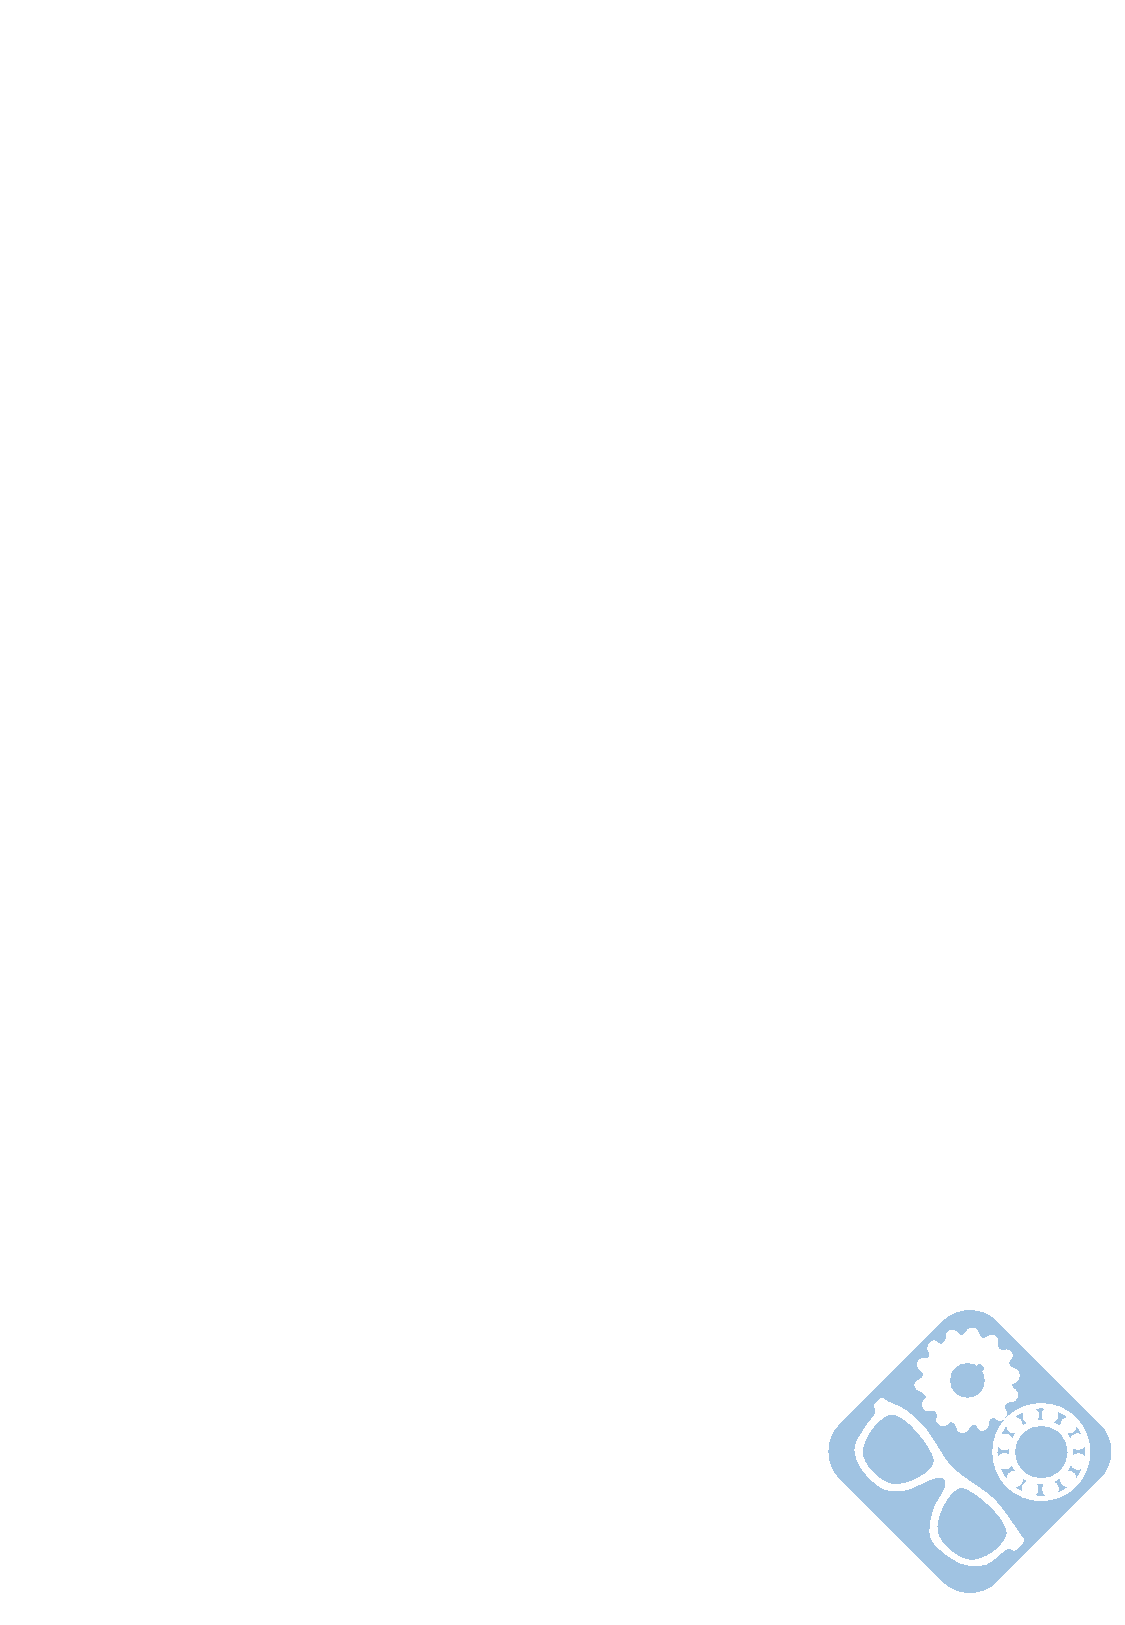
\includegraphics[width=\paperwidth,height=\paperheight,%
keepaspectratio]{../../../img/fond4}%
\end{center}
\vfill
}}}

\begin{document}

\pagestyle{empty}

\AddToShipoutPicture*{\BackgroundPic}


\includegraphics[width=2cm]{../../../img/logo}

\Huge{DS \numero - \sujet}

\vspace{1cm}

\ifdef{\prive}{\begin{center}\colorbox{danger}{\Huge{Avec Correction}}\end{center}}{}

\begin{center}
\centering\huge{PTSI}
\end{center}

\vspace{2cm}


\begin{center}
\centering\Large{\jour}
\end{center}

\vspace{2cm}

\normalsize

\tableofcontents

\newpage

\AddToShipoutPicture{\BackgroundPicdeux}

\pagestyle{fancy}

\begin{center}
\Huge \sujet
\end{center}


\normalsize


\section{Mise en situation et contexte de l'étude}

\paragraph{Objectif :} S'approprier le contexte de l'étude et établir un modèle de comportement du système.

\begin{figure}[ht!]
\begin{minipage}{0.65\linewidth}
\subsection{Gus : Une révolution dans le déplacement}

Depuis plus de six ans la société OPUS TECHNOLOGIES conçoit, met au point et fabrique un fauteuil électrique particulièrement innovant, appelé GUS, acronyme de Gyropode Utilitaire et Sportif, figure \ref{fig02}.

~\

Son design, son principe de fonctionnement basé sur une solution de type Gyropode et sa maniabilité sont pensés pour modifier le regard de chacun sur les handicapés en fauteuil roulant et plus généralement le regard que nous portons sur le handicap.

~\

Le GUS est fabriqué en France. 80 \% de ses composants sont d'origine
Française et une part significative des opérations nécessaires à sa
fabrication est réalisée par des personnes en situation de handicap, ce
qui représente une réelle fierté pour l'entreprise.
\end{minipage}\hfill
\begin{minipage}{0.3\linewidth}
\centering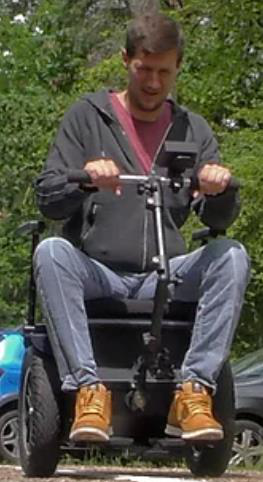
\includegraphics[width=0.9\linewidth]{img/fig01.png}
\caption{\label{fig01} Personne utilisant le fauteuil GUS}
\end{minipage}
\end{figure}

\begin{figure}[ht!]
\centering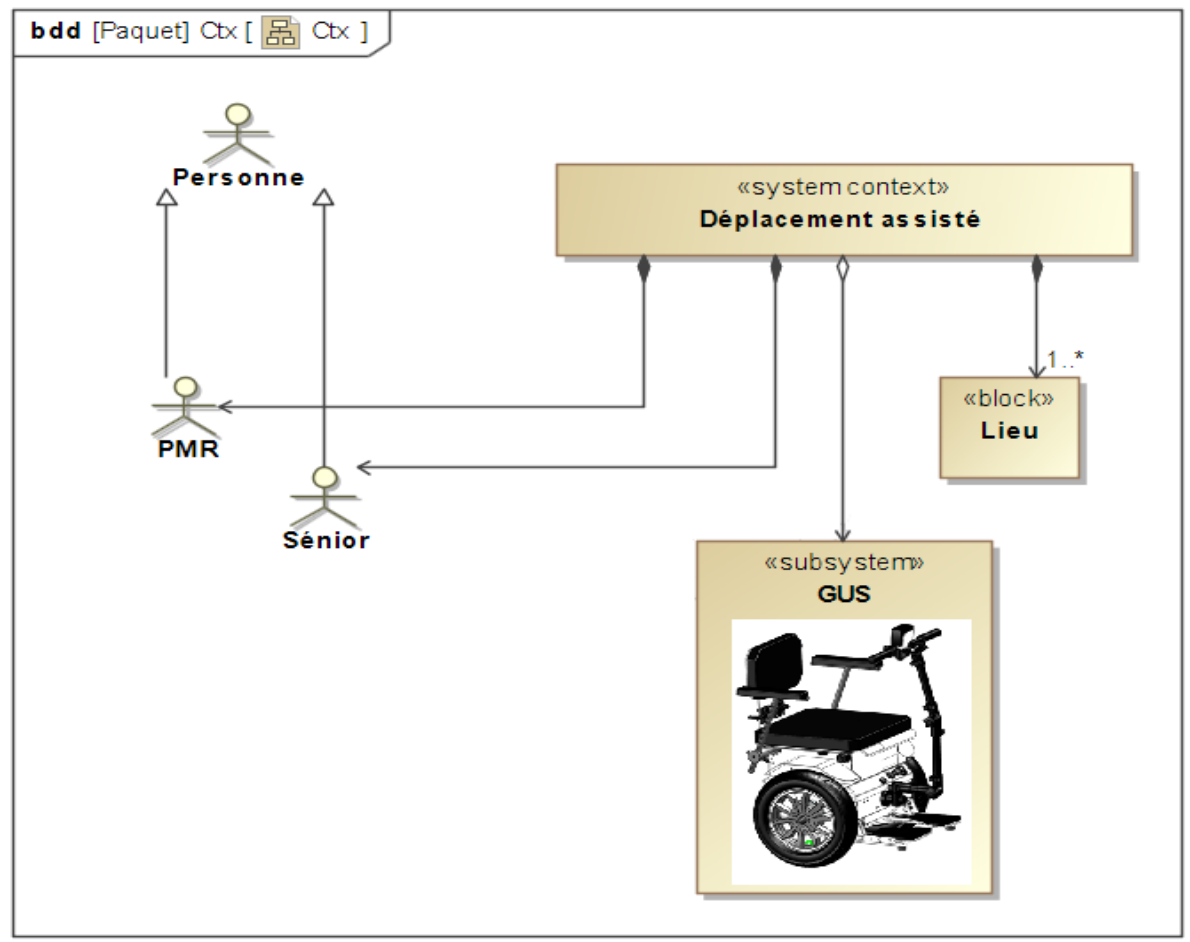
\includegraphics[width=0.6\linewidth]{img/fig02.png}
\caption{\label{fig02} Diagramme de contexte}
\end{figure}

Enfin, un des modèles économiques de distribution de ce fauteuil est
basé sur la vente par des personnes déjà utilisatrices d'un GUS. Cette
proximité permet de mieux appréhender et de mieux répondre aux besoins des personnes ayant une nécessité d'assistance dans leurs déplacements quotidiens. Elle permet également de faire remonter les réalités et les différentes problématiques du terrain à l'équipe en charge de la conception.

En Septembre 2021, les premiers exemplaires sont désormais en pré-commande et les retours sont d'ores et déjà très positifs.

\subsection{Contexte de l'étude}

L'étude se situe donc dans un contexte de prévente autour des solutions technologiques retenues après six ans de recherche et développement. Comme toute démarche technologique et économique, ces solutions sont le résultat permanent d'un compromis entre prix et performances.

\subsection{Présentation du principe de fonctionnement du GUS}

\begin{figure}[ht!]
\begin{minipage}{0.6\linewidth}
Le GUS est basé sur une solution de type Gyropode. La figure \ref{fig03} indique clairement que la particularité du GUS est de ne disposer que de deux roues motrices sans aucun autre point de stabilisation lors des déplacements. Son centre de gravité se situe au-dessus de l'axe des roues.

Cette solution est nativement instable. Un accéléromètre et un gyromètre intégrés à la carte de commande permettent de déterminer en continu l'inclinaison du GUS. Les boucles d'asservissement régulent d'une part la stabilité et d'autre part le déplacement de ce dernier. Il repose en cela sur le principe de fonctionnement d'un pendule inversé.

L'équilibre à l'arrêt repose sur un système de béquillage organisé autour de trois plots qui viennent stabiliser le fauteuil (figure \ref{fig04}). Ces trois plots sont mis en mouvement par l'intermédiaire d'une fourche actionnée par un vérin. Un second vérin vient renforcer le positionnement de la fourche, une fois cette dernière mise en place.
\end{minipage}
\hfill
\begin{minipage}{0.35\linewidth}
\centering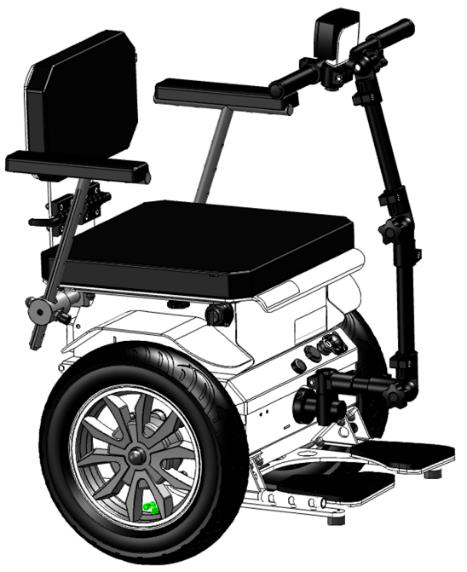
\includegraphics[width=0.8\linewidth]{img/fig03}
\caption{\label{fig03}Modèle 3D}
\end{minipage}
\end{figure}


\begin{figure}[ht!]
\begin{minipage}{0.5\linewidth}
\centering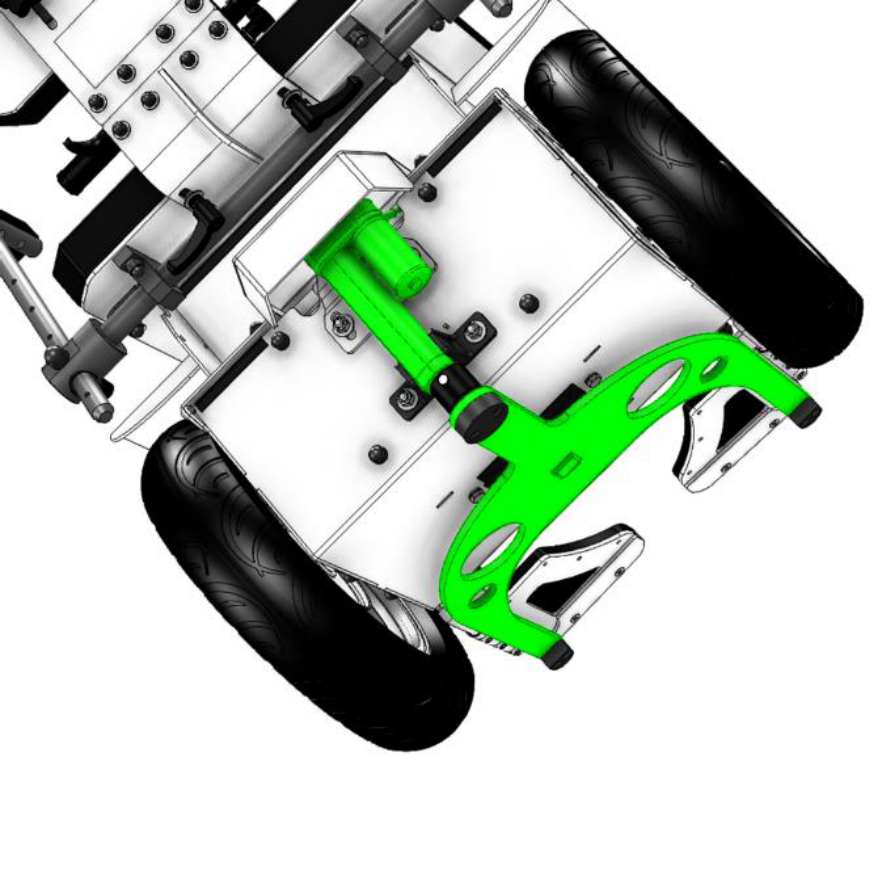
\includegraphics[width=0.8\linewidth]{img/fig04}
\caption{\label{fig04}Système de béquillage}
\end{minipage}
\hfill
\begin{minipage}{0.45\linewidth}
Lors du déplacement, le GUS commence à retirer le système de béquillage et met en place immédiatement le système d'équilibrage et de pilotage. Le béquillage est remis en position lors de l'arrêt du GUS. De plus, si un évènement quelconque risquant de nuire à l'équilibre du GUS est détecté
pendant la phase de fonctionnement, le système de béquillage est immédiatement mis en place empêchant ainsi toute perte d'équilibre.
\end{minipage}
\end{figure}

\subsection{Analyse du diagramme partiel des exigences}

\question{A la lecture du diagramme des exigences, disponible sur le document technique DT1, indiquer quelles sont les performances attendues en termes d'autonomie, de vitesse maximale en fonctionnement et d'encombrement nécessaire au sol. Selon vous, l'autonomie parait-elle suffisante dans les trajets du quotidien ?}

\subsection{Diagrammes états transitions du fonctionnement du GUS}

Le fonctionnement du GUS commence lors de l'installation de la personne sur le fauteuil. Cette action déclenche l'événement \textbf{ON}.

Il se termine lorsque la personne quitte le fauteuil. Cette action déclenche l'événement \textbf{OFF}.

En situation de fonctionnement, on distingue deux modes principaux. Ils correspondent à des états dans lequel le GUS peut se trouver.
\begin{itemize}
 \item Un mode \textbf{Arrêt} dans lequel le béquillage est actif et durant lequel les asservissements sont désactivés. Ce mode ne consomme quasiment pas d'énergie car seule la veille de la carte de commande est activée.
 \item Un mode \textbf{Marche} dans lequel le béquillage est inactif et durant lequel les asservissements sont actifs. Ce mode correspond au fonctionnement normal du fauteuil et autorise tous les déplacements en assurant l'équilibre du fauteuil. Lors de ce mode, les paramètres du GUS
sont surveillés en temps réel. Le système de béquillage se met en fonctionnement, désactivant les asservissements, si au moins un des paramètres indique qu'un risque de perte d'équilibre est détecté. GUS passe alors en mode \textbf{Arrêt}.
\end{itemize}

~\

Les événements à prendre en considération sont :
\begin{itemize}
 \item \textbf{ON} : Début d'utilisation du fauteuil lors de l'installation de la personne,
 \item \textbf{OFF} : Fin d'utilisation du fauteuil et retrait de la personne.
\end{itemize}
\begin{itemize}
 \item \textbf{CMB} : Commande Manuelle de Béquillage (béquillage actif),
 \item \textbf{CMD} : Commande Manuelle de Dé-béquillage (béquillage inactif),
 \item \textbf{CAB} : Commande Automatique de Béquillage (béquillage actif)
\end{itemize}

\question{A l'aide des informations précédentes, compléter le document réponse, correspondant au modèle de comportement macroscopique régissant le fonctionnement du GUS.}

En réalité, lors de l'activation du mode \textbf{Marche}, deux sous-ensembles sont activés en même temps, chacun d'entre eux ayant une fonction bien précise. Le premier de nom \textbf{Déplacement/Asservissement} gère l'équilibre du fauteuil et son déplacement suivant les souhaits de la personne. Le second nommé \textbf{Surveillance} veille au respect des paramètres critiques du GUS et déclenche l'évènement CAB si nécessaire, évitant ainsi toute chute accidentelle.

\question{A l'aide de la description de l'état \textbf{Marche}, compléter le document réponse, correspondant au modèle de comportement complet régissant le fonctionnement du GUS.}

\subsection{Conclusion}

\question{Vis-à-vis de la modélisation comportementale abordée et sachant que l'opération de béquillage se fait en moins de 200 ms, conclure sur le respect des exigences 1.2 et 1.2.1 du document technique DT1.}

\section{Étude de la motorisation du GUS}

\paragraph{Objectif :} Vérifier la réalisation de l'exigence 1.4.1 concernant la validation de la vitesse maximale et estimer le contenu spectral des signaux engendrés par l'utilisation de hacheurs quatre quadrants afin de préparer la validation de l'exigence 1.6.3.

\subsection{Présentation générale}

Lors des différentes phases de conception, plusieurs types de motorisation ont été analysés et testés. Après plusieurs essais, le choix s'est finalement porté sur une motorisation à base de moteurs à courant continu, associés à leurs réducteurs intégrés, spécialement créés pour ce type d'application. Ce choix impose également des variateurs de vitesse compatibles avec ce type de motorisation.

Le diagramme de bloc (BDD) partiel du GUS et le diagramme de blocs internes (IBD) relatifs à la partie \textbf{Motorisation} sont donnés sur le document technique DT2.

\question{Sur le document réponse, compléter les différents types de flux d'énergie échangés au sein du bloc Motorisation.}

~\

Les nouvelles versions du GUS sont ainsi équipées de deux moto-réducteurs à courant continu, d'origine chinoise, de référence DM088110-036-02. L'intégralité de la documentation disponible pour la série de moteurs, dont fait partie celui retenu pour le GUS, est fournie sur le document
technique DT3.

\subsection{Validation du choix du moto-réducteur en vitesse de rotation}

Pour rappel, le diagramme d'exigence indique que la vitesse maximale en charge en l'absence de toute modulation doit être supérieure à $15km\cdot h^{-1}$.

\question{Sachant que le diamètre extérieur des roues est $D_R=42cm$, montrer que le choix de ce moto-réducteur permet de satisfaire l'exigence de vitesse maximale en charge, autorisant des petits mouvements rapides d'équilibrage.}

\subsection{Obtention du modèle du moteur à courant continu composant le moto-réducteur}

Le moto-réducteur est composé d'une machine à courant continu et d'un réducteur à dentures obliques de réduction $R_{red}=17$.

On néglige dans cette partie l'inductance $L$ du moteur et une mesure préparatoire a montré que la valeur de la résistance $R$ de l'induit est $R=0,4\Omega$. On réalise un essai à vide dans les conditions
décrites sur la documentation technique du moto-réducteur afin de déterminer le couple de perte de l'ensemble moto-réducteur.

La puissance électrique à vide s'exprime comme la somme des pertes:
\begin{itemize}
 \item Joule,
 \item collectives, composées des pertes mécaniques et des pertes magnétiques $C_p\cdot \Omega_{vide}$.
\end{itemize} 

\question{Déterminer la valeur du couple de perte $C_p$ du moto-réducteur lors de l'essai à vide sous tension nominale, soit $U_0=36V$.}

\question{A l'aide du document technique DT3, déterminer le couple nominal en charge du moto-réducteur, le couple maximal admissible et le rendement nominal $\eta=\dfrac{P_{charge}}{P_{absorbee}}$. Conclure sur la valeur du rendement nominal de ce moto-réducteur.}

~\

Par la suite, on néglige le couple de perte et donc le courant appelé à vide en supposant que ce dernier est négligeable devant le courant appelé en charge.

\question{Déterminer la vitesse à vide $\Omega_{M_{vide}}$ du moteur à courant continu composant le moto-réducteur. En négligeant le courant appelé à vide, en déduire la valeur du coefficient $K_E$ en $V\cdot rad^{-1}\cdot s$ tel que $E=K_E\cdot \Omega_M$.}

\subsection{Validation du choix du moto-réducteur en couple maximal}

On suppose désormais que le couple maximal disponible sur l'arbre de chaque moto-réducteur est égal à $C_{max}=48N\cdot m$.

~\

La validation du couple maximal se fait dans les conditions suivantes :
\begin{itemize}
 \item Le fauteuil avec son passager est immobile mais le béquillage n'est pas actif,
 \item Le passager de masse $m_{Passager}$ et dont le centre de masse $G_P$, est situé exactement dans l'axe des roues, se penche lentement en avant d'un angle $\delta$ par rapport à la verticale,
 \item Accélération de la pesanteur : $g=9.81m\cdot s^{-2}$.
\end{itemize}

On pose $\ell$, distance entre la position du centre de gravité $G_G$ du GUS et $G_P$, la position du centre de gravité du passager.

Un premier modèle, dans lequel la somme des couples disponibles $C_{Total}$, produit par les deux moto-réducteurs, est utilisée uniquement pour maintenir l'équilibre du passager permet d'obtenir
la relation suivante :
$$C_{Total}=m_{passager}\cdot g\cdot \ell\cdot sin\delta$$

\question{Déterminer l'expression de l'angle $\delta$ à partir duquel il n'est plus possible de maintenir l'équilibre. Faire l'application numérique sachant que la masse maximale du passager $m_{passager_{max}}=100kg$ et que la distance $\ell$ est prise égale à $0,5m$. Comment
évolue cet angle si la masse du passager diminue ? Conclure sur la valeur du couple maximal et l'angle de débattement.}

\subsection{Validation du type de variateur de vitesse}

\begin{figure}[ht!]
\begin{minipage}{0.6\linewidth}
Chaque moto-réducteur est piloté par un \textbf{ConVertisseur Statique d'énergie (CVS)} de type hacheur quatre quadrants (figure \ref{fig05}).

Chaque interrupteur $K_i$ est composé d'un transistor $T_i$, de type MOSFET Canal N, et d'une diode de puissance $D_i$ montée en anti parallèle.

Le pilotage de chaque interrupteur provient du bloc \textbf{Carte de traitement}.
\end{minipage}
\hfill
\begin{minipage}{0.35\linewidth}
\centering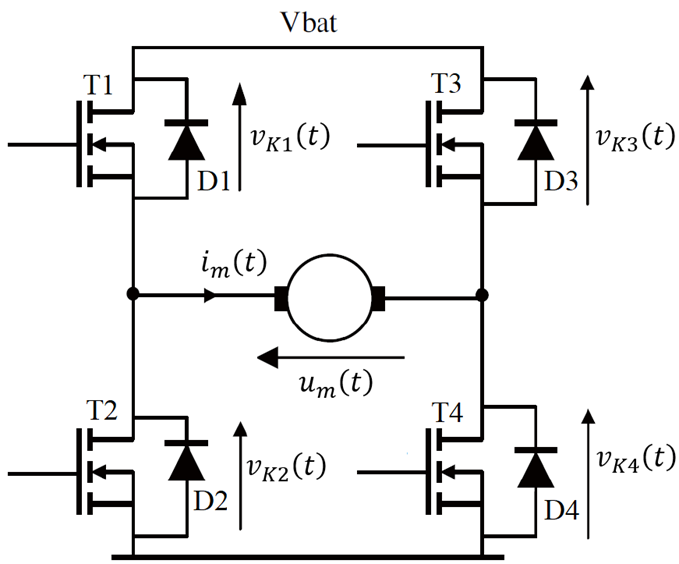
\includegraphics[width=0.8\linewidth]{img/fig05}
\caption{\label{fig05}Hacheur quatre quadrants}
\end{minipage}
\end{figure}

\question{Sur le document réponse, représentant l'IBD de la partie Motorisation présentée sur le document technique DT2, faire apparaitre le flux issu du bloc \textbf{Carte de traitement} et entrant dans le \textbf{ConVertisseur Statique d'énergie}. Indiquer quelle est la nature de ce flux. De combien de composantes ce flux est-il constitué ?}

~\

Dans certaines configurations de fonctionnement, il est possible que le GUS devienne générateur en phase de descente.

\question{Justifier alors le choix retenu pour le type de \textbf{ConVertisseur Statique d'énergie}. Indiquer combien de segments de fonctionnement doit posséder chaque interrupteur $K_I$ et préciser lesquels.}

~\

Dans chaque interrupteur $K_i$, le transistor $T_i$ est un transistor MOSFET de référence IRF1405 dont la documentation partielle est fournie sur le document technique DT4.

Lors d'un fonctionnement en pleine charge, le moto-réducteur peut appeler un courant $I_{M_{max}}$ de 34 A sous une tension de la batterie de 36 V.

\newpage

Pour un composant donné, on définit le coefficient de sécurité $s$ d'une grandeur $g$ comme étant le rapport entre la valeur numérique $g_{num}$ de cette grandeur et la valeur maximale $g_{max}$ que peut supporter ce composant pour cette grandeur $g$ sans détérioration.

$$s=\dfrac{g_{num}}{g_{max}}$$

\question{Pour le transistor $T_i$, composant l'interrupteur $K_i$, déterminer les coefficients de sécurité en courant et en tension. Valider le choix de ce transistor.}

\subsection{Câblage moto-réducteurs et variateurs}

Le câblage entre les variateurs ($H4Q_{Droit}$ et $H4Q_{Gauche}$) et les moto-réducteurs ($M_{Droit}$ et $M_{Gauche}$) est réalisé de manière à obtenir les résultats suivants.

\begin{itemize}
 \item En marche avant, les deux moteurs ont une tension positive à leurs bornes.
 \item En marche arrière, les deux moteurs ont une tension négative à leurs bornes.
\end{itemize}

En phase de rotation, tous les cas de figure peuvent se présenter suivant que le fauteuil pivote sur son centre ou qu'il réalise un virage en marche avant ou en marche arrière.

\subsection{Commandes des variateurs}

Pour le type de variateur retenu, deux types de commandes différentes sont possibles.

\begin{itemize}
 \item Une première nommée : Commande unipolaire ou séquentielle,
 \item Une seconde nommée : Commande bipolaire ou continue.
\end{itemize}

Le choix privilégié par les concepteurs est une commande de type unipolaire. Dans ce type de commande, deux interrupteurs sont pilotés par période de hachage $T$ alors qu'en commande bipolaire, les quatre interrupteurs sont pilotés par période de hachage $T$.

Pour la suite de l'étude, on se place en marche avant, à vitesse constante, et on ne s'intéresse qu'au moto-réducteur droit $M_{Droit}$, piloté par le variateur $H4Q_{Droit}$.

\begin{figure}[ht!]
\begin{minipage}{0.65\linewidth}
On fait l'hypothèse que dans la configuration étudiée le fonctionnement du ConVertisseur Statique d'énergie est en mode continu.

Dans ce cas de figure, on cherche ainsi à obtenir une tension moyenne positive aux bornes du moto-réducteur conforme à celle de la figure \ref{fig06}.
\end{minipage}\hfill
\begin{minipage}{0.3\linewidth}
\centering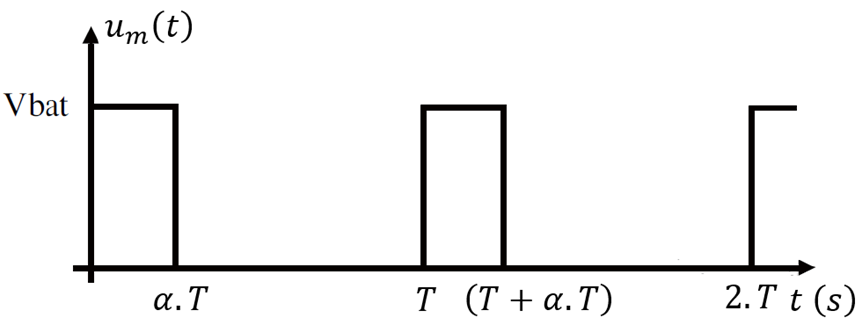
\includegraphics[width=0.9\linewidth]{img/fig06.png}
\caption{\label{fig06} Tension aux bornes du moto-réducteur $M_{Droit}$}
\end{minipage}
\end{figure}

La période de hachage $T$ se décompose en deux parties. Une première de 0 à $\alpha\cdot T$ et une seconde de $\alpha\cdot T$ à $T$.

On entend par composant actif, un composant qui au cours de la période de hachage $T$ change d'état dans son fonctionnement, c'est-à-dire passe de l'état bloqué à l'état saturé (ou passant) ou l'inverse.

\newpage

Pour obtenir la tension souhaitée, on pilote en permanence la fermeture de l'interrupteur $K_4$ et on hache la tension grâce au pilotage de l'interrupteur $K_1$ qui est commandé à la fermeture lors de 
la première partie de la période, soit de 0 à $\alpha\cdot T$ et à l'ouverture lors de la seconde partie de la période, soit de $\alpha\cdot T$ à $T$.

\question{Dans le cas de figure étudié, indiquer quels sont les composants actifs en complétant le tableau du document réponse. En se focalisant uniquement sur les composants actifs et en remplaçant les composants inactifs soit par des circuits ouverts, soit par des circuits fermés, préciser à quelle structure de hacheur se ramène ce cas de
figure.}

\question{A partir de la tension aux bornes du moto-réducteur, représentée figure \ref{fig06}, déterminer la valeur moyenne $<U_m>$ de cette tension.}

\section{Approche MBD - Model Based Design : Conception basée sur le
modèle}

\paragraph{Objectif :} Mettre au point un modèle de simulation pour prédire le fonctionnement du GUS et valider le choix technologique du moto-réducteur ainsi que la trajectoire obtenue lors d'une commande différentielle des hacheurs.

\subsection{Présentation générale du modèle}

Les avancés de la simulation multi-physique permettent de prédire certains comportements et ainsi de valider certains choix technologiques afin de réduire les coûts d'étude et in fine les temps de conception. Cette approche est nommée Model Based Design ou Conception basée sur le
modèle.

Dans le cas du GUS, un modèle multiphysique du fonctionnement en boucle ouverte pour la partie chaîne d'énergie est conçu. Il est reproduit sur le document technique DT5. Ce dernier contient déjà des informations issues, soit des études précédentes, soit des différentes documentations des composants retenus dans la conception.

Les éléments suivants sont renseignés dans le modèle.

~\

Pour les moto-réducteurs :
\begin{itemize}
 \item Coefficient $K_E$,
 \item Résistance interne $R$,
 \item Inductance interne et inductance de lissage $L$,
 \item Courant à vide sous tension nominale ($V_{bat}= 36V$) $I_0=3A$,
 \item Coefficient de réduction du réducteur intégré $R_{red}=17$.
\end{itemize}

~\

Pour les roues :
\begin{itemize}
 \item Diamètre de la roue : $D_R=42cm$,
\end{itemize}

\newpage

Pour la batterie :
\begin{itemize}
 \item Type : Lithium Ion,
 \item Charge de la batterie $100\%$,
 \item Tension à vide $V_{bat0}=38V$ et en fonctionnement $V_{bat}=36V$,
 \item Capacité : $28Ah$.
\end{itemize}

~\

Les hacheurs quatre quadrants sont remplacés par des hacheurs équivalents dans le cas de figure considéré et les éléments suivants sont renseignés dans le modèle:
\begin{itemize}
 \item Type d'interrupteur commandé : MOSFET Canal N à enrichissement,
 \item Diode de puissance.
\end{itemize}

~

Pour le lien entre les sorties des générateurs DC/PWM et les entrées des hacheurs :
\begin{itemize}
 \item Les signaux de commande des hacheurs sont adaptés pour être compatibles avec les sorties des générateurs DC/PWM.
\end{itemize}

~\

Pour le générateur PWM :
\begin{itemize}
 \item La fréquence de pilotage des interrupteurs est égale à $20kHz$,
 \item Le paramètre d'entrée du générateur PWM est la valeur du rapport cyclique $\alpha$.
\end{itemize}

\subsection{Première utilisation de l'approche MBD}

\subsubsection{Détermination de l'effort résistant}

La validation du courant moteur se fait dans les conditions suivantes (figure \ref{fig07}) :

\begin{figure}[ht!]
\begin{minipage}{0.5\linewidth}
Pour le fauteuil et son passager :
\begin{itemize}
 \item Masse du fauteuil avec son passager : $M=160Kg$,
 \item Centre de gravité du fauteuil avec son passager : Point $G$,
 \item Accélération de la pesanteur : $g~=~9.81m\cdot s^{-2}$. 
\end{itemize}

Pour la route :
\begin{itemize}
 \item Pente de la route importante,
 \item Route en mauvais état avec un coefficient de roulement élevé.
\end{itemize}
\end{minipage}\hfill
\begin{minipage}{0.45\linewidth}
\centering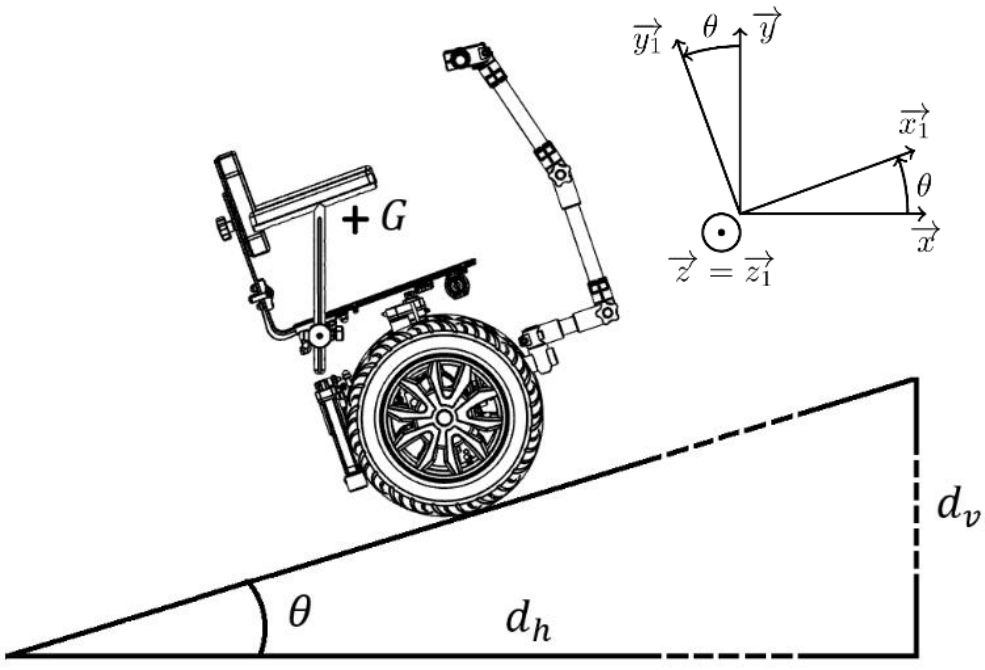
\includegraphics[width=0.9\linewidth]{img/fig07}
\caption{\label{fig07}Le GUS sur une route en pente}
\end{minipage}
\end{figure}

Pour la trajectoire :
\begin{itemize}
 \item Déplacement rectiligne le long de la route (en pente) à vitesse constante.
\end{itemize}

\newpage

Hypothèse supplémentaire :
\begin{itemize}
 \item Roulement sans glissement aux deux points de contact des roues avec le sol,
 \item Compte tenu des faibles vitesses mises en jeu, l'effort résistant lié aux forces aérodynamiques s'exerçant sur le fauteuil et son passager est négligé.
\end{itemize}

\question{A partir des conditions énoncées, justifier la pertinence de la prise en compte d'une hypothèse de modélisation plane.}

~\

On définit la pente d'une route comme le quotient de la distance $d_v$ par la distance $d_h$.

\question{Déterminer l'expression de l'angle $\theta$ en fonction des paramètres $d_v$ et $d_h$.

En déduire la valeur de cet angle si la pente de la route est de $\dfrac{d_v}{d_h}=10\%$.}

~\

On isole l'ensemble {Fauteuil + Passager}. Le torseur de l'action de la pesanteur sur cet ensemble au point G, centre de gravité du {Fauteuil + Passager} s'écrit :
$$\left\{T_{Pes\rightarrow {Fauteuil+Passager}}\right\}=\left\{\begin{array}{c}-M\cdot g\cdot \vec{y}\\\vec{0}
\end{array}
\right\}_G$$

Le torseur de l'action du sol sur cet ensemble au point M, point de contact), s'écrit :
$$\left\{T_{Sol\rightarrow {Fauteuil+Passager}}\right\}=\left\{\begin{array}{c}F_{RT} \cdot \vec{x_1}+ F_{RN}\cdot \vec{y_1}\\\vec{0}
\end{array}
\right\}_M$$
déformation des pneus
\question{Déterminer l'expression de l'effort résistant tangentiel $F_{RT}$ lié à l'action de la pesanteur dans le repère de la route. Faire l'application numérique dans le cas retenu pour la simulation.}

~\

En prenant en compte les efforts liées à la résistance au roulement, on définit la force résistante sur le sol comme :$\overrightarrow{F_{Roul}}\cdot\vec{x_1}=-M\cdot g\cdot C_{rr}\cdot cos(\theta)$.

\question{Calculer la valeur numérique de l'effort résistant lié à la résistance des pneus, si l'on considère que $C_{rr}=0,02$. Cet effort peut-il être négligé devant le précédent ?}

\subsection{Seconde utilisation de l'approche MBD : Détermination des distances parcourues}

On se place désormais sur une route horizontale en bitume. La somme des efforts résistants est dans ce cas très faible et on choisit de la limiter à $10N$ par moto-réducteur, sans tenir compte d'un éventuel déséquilibre. On cherche à tracer la trajectoire lorsque le manche de pilotage est légèrement incliné vers la gauche, ce qui implique que les commandes de pilotage sur les deux moto-réducteurs ne sont plus identiques. On se place dans l'hypothèse suivante :
\begin{itemize}
 \item Pour le rapport cyclique de pilotage de la roue droite : $\alpha_d= 0,36$,
 \item Pour le rapport cyclique de pilotage de la roue gauche : $\alpha_g=0,28$.
\end{itemize}

On fait l'hypothèse d'un roulement sans glissement pour les deux roues du GUS. Le modèle permet d'obtenir les distances parcourues par ces dernières.

\subsubsection{Obtention des distances parcourues}

Au terme d'une simulation représentant une durée simulée de 10 secondes, on obtient le chronogramme représentant les déplacements effectués par chacune des deux roues (figure \ref{fig10}).

\begin{figure}[ht!]
\centering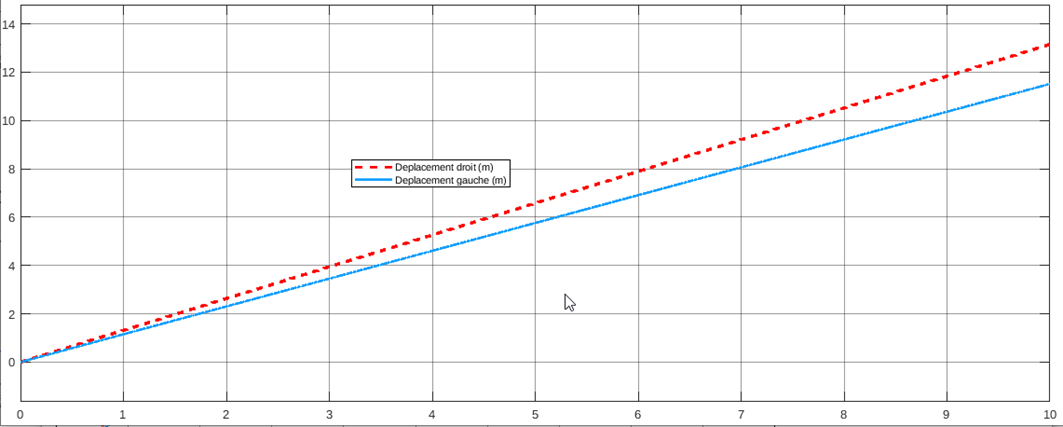
\includegraphics[width=\linewidth]{img/fig10}
\caption{\label{fig10}Résultats de la simulation}
\end{figure}

\begin{figure}[ht!]
\begin{minipage}{0.55\linewidth}
Sur ce chronogramme, au bout de 10 secondes, on peut lire les informations suivantes.
\begin{itemize}
 \item Pour le déplacement droit : $d_d=13,15m$ ;
 \item Pour le déplacement gauche : $d_g=11,52m$.
\end{itemize}

La largeur du fauteuil et de son passager est $d_\ell=0,63m$.

Pour des raisons de symétrie, le centre de gravité du fauteuil et du passager se situe à la verticale du centre du fauteuil.
\end{minipage}\hfill
\begin{minipage}{0.55\linewidth}
\centering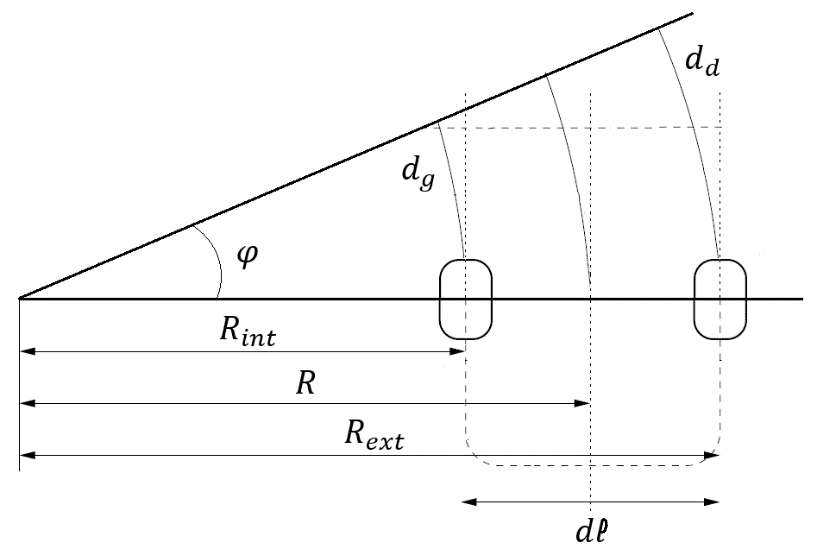
\includegraphics[width=0.8\linewidth]{img/fig11}
\caption{\label{fig11}Déplacement du GUS}
\end{minipage}
\end{figure}

La figure \ref{fig11} précise les notations utilisées. La trajectoire obtenue est un cercle de rayon $R$.

\question{Donner l'expression de l'angle $\varphi$ en fonction de $d_d$, $d_g$ et $d_\ell$. Faire l'application numérique.}

\question{Montrer que le rayon de giration $R$ s'écrit : $R=\dfrac{d_\ell}{2}\cdot\dfrac{d_d+d_g}{d_d-d_g}$. Faire l'application numérique et en déduire la distance parcourue $d_p$.}

\newpage

\subsubsection{Tracé de la trajectoire obtenue}

A partir des expressions mathématiques obtenues, une fonction informatique \texttt{trajectoireC()} est écrite pour faire afficher la trajectoire effectuée. Le résultat de cette fonction est l'affichage d'une courbe représentant la trajectoire effectuée.

\question{Sur le document réponse, représentant la trajectoire effectuée, indiquer la position du centre $O$ du cercle, la longueur $d_p$, le rayon $R$, le point de départ $A$, le sens du parcours du fauteuil et de son passager et le point d'arrivée $B$.}

\section{Amélioration du confort du passager}

\paragraph{Objectif :} Valider les solutions technologiques mise en place pour améliorer le confort du passager et vérifier la réalisation des exigences 1.5.1 et 1.5.2.

\subsection{Présentation}

\begin{figure}[ht!]
\begin{minipage}{0.55\linewidth}
Le dossier du GUS est présenté sur la figure \ref{fig12}.

Il comporte deux parties spécifiques permettant d'une part de régler la hauteur du dosseret (exigence 1.5.1) et d'autre part de plier le dosseret grâce à un système de charnières afin de réduire l'encombrement notamment, lors des phases de transport dans un véhicule (exigence 1.5.2).

\subsection{Étude du réglage du dosseret en hauteur}

\subsubsection{Détermination de la liaison équivalente}

On s'intéresse à la liaison équivalente entre la Plaque dossier (1) et la Tôle haute (0) considérée comme le bâti.

\begin{itemize}
 \item Chacune des deux liaisons entre (0) et (1) peut être modélisée par une liaison pivot glissant:
 \begin{itemize}
  \item Une première d'axe $(A,\vec{z})$,
  \item Une seconde d'axe $(B,\vec{z})$.
  \end{itemize}
 \item On pose : $\overrightarrow{AB}=L\cdot \vec{y}$
\end{itemize}
\end{minipage}\hfill
\begin{minipage}{0.55\linewidth}
\centering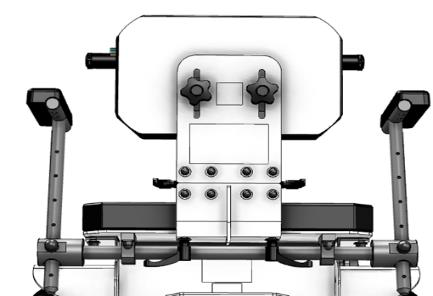
\includegraphics[width=0.8\linewidth]{img/fig12}
\caption{\label{fig12}Dossier du GUS}
\centering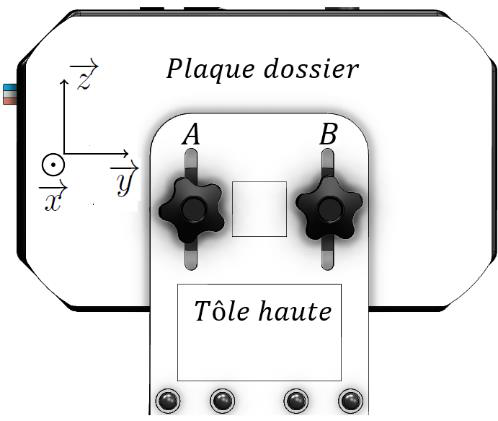
\includegraphics[width=0.8\linewidth]{img/fig13}
\caption{\label{fig13}Liaison (1) - (0)}
\end{minipage}
\end{figure}

\question{Établir le graphe de structure puis le schéma cinématique de l'ensemble.}

\question{Établir la liaison équivalente entre la Plaque dossier (1) et la Tôle haute (0).}

\question{Déterminer le degré d'hyperstaticité de cette solution. Quelles sont les contraintes géométriques à respecter pour sa réalisation ?}

\subsubsection{Maintien en position du dosseret et validation de l'exigence 1.5.1}

L'étude de la solution précédente autorise encore le déplacement de la Plaque dossier (1) par rapport à la Tôle haute (0).

\question{Indiquer de quelle manière, le maintien en position de la Plaque dossier (1) par rapport à la Tôle haute (0) est assuré et conclure sur le respect de l'exigence 1.5.1.}

\subsection{Étude du pliage du dossier}

Les deux charnières utilisées dans la réalisation du dosseret permettent de rapidement replier le dossier sur lui-même afin de réduire l'encombrement notamment lors des phases de transport en voiture.

Les charnières retenues pour cette application sont des charnières CFA65-ERS-SH6 de la société Elesa+Ganter®. Il s'agit de charnières avec système de blocage à friction (figure \ref{fig14}). Une documentation partielle est disponible sur le document technique DT6.

\subsubsection{Modélisation du couple de serrage des charnières}

On cherche à modéliser le couple de serrage de ces charnières à friction en s'intéressant en premier à la friction entre deux éléments de la charnière.

\begin{figure}[ht!]
\begin{minipage}{0.55\linewidth}
La détermination se fait dans les conditions suivantes :
\begin{itemize}
 \item L'effort presseur est modélisé par un glisseur de résultante $\overrightarrow{R_{2\rightarrow 1}}=-F\cdot \vec{z}$,
 \item La surface de contact entre les deux parties est un anneau
d'angle $2\cdot\pi$, de rayon intérieur $r_{int}$ et de rayon extérieur $r_{ext}$,
 \item On note $p_n$ la pression de contact normale, supposée uniformément répartie,
 \item On note $p_t$ la pression tangentielle. La norme de la pression tangentielle est obtenue à partir de la norme de la pression normale et du coefficient de frottement $f$, soit $\|p_t\|=f\cdot p_n$,
 \item L'action de la pesanteur est négligée devant les autres actions mécaniques.
\end{itemize}
\end{minipage}\hfill
\begin{minipage}{0.55\linewidth}
\centering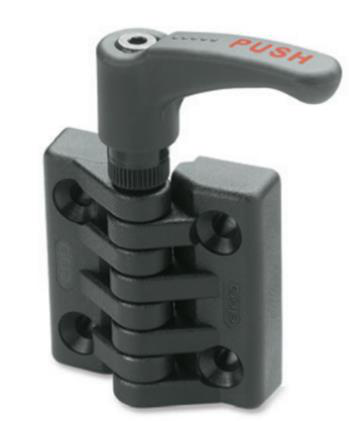
\includegraphics[width=0.8\linewidth]{img/fig14}
\caption{\label{fig14}Charnière CFA65-ERS-SH6}
\end{minipage}
\end{figure}

\begin{figure}[ht!]
\begin{minipage}{0.55\linewidth}
La détermination se fait dans les conditions suivantes :
Avec les hypothèses précédentes, on suppose désormais que le modèle de pression au point M, point quelconque de l'anneau s'écrit :

$$\overrightarrow{dF_{2\rightarrow 1}}=(-p_n\cdot \vec{z}+p_t\cdot \vec{v})\cdot ds\ avec\ p_t=f\cdot p_n$$

Le paramétrage du modèle de calcul est donné sur la figure \ref{fig15}.

\begin{itemize}
 \item On pose $\overrightarrow{OM}=r\cdot \vec{u}$
\end{itemize}

\end{minipage}\hfill
\begin{minipage}{0.55\linewidth}
\centering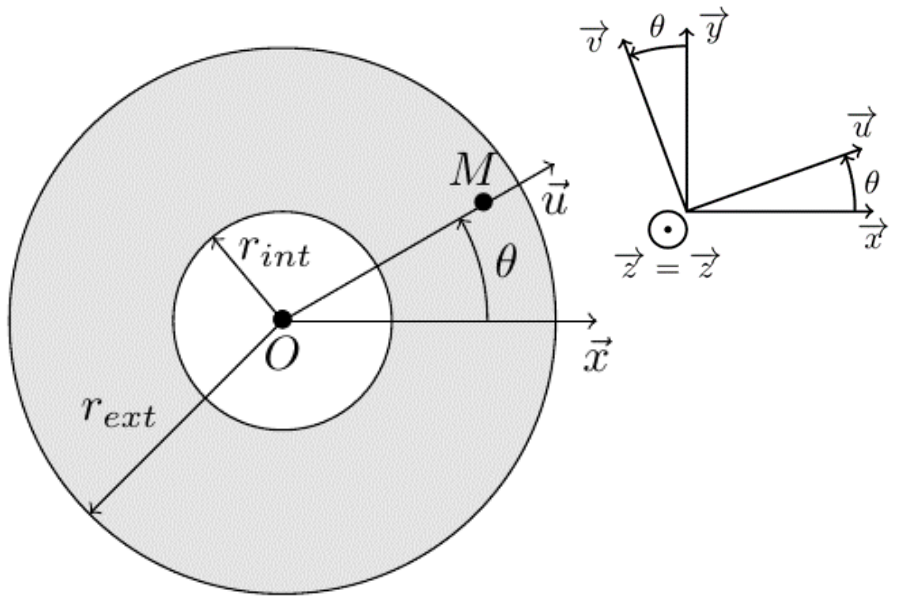
\includegraphics[width=0.8\linewidth]{img/fig15}
\caption{\label{fig15}Paramétrage du modèle de calcul}
\end{minipage}
\end{figure}

\subsubsection{Expression du torseur de l'action mécanique au point O}

On cherche à déterminer le modèle global de l'action mécanique en $O$ à partir du modèle local des actions mécaniques. Pour cela, on rappelle que 

$$\left\{T_{2\rightarrow 1}\right\}=\left\{\begin{array}{c}\overrightarrow{R_{2\rightarrow 1}}\\\overrightarrow{M_{O,2\rightarrow 1}}\end{array}\right\}_O=\left\{\begin{array}{c}\int_{\forall M\in S} \overrightarrow{dF_{2\rightarrow 1}(M)}\\\int_{\forall M\in S} \overrightarrow{OM}\wedge\overrightarrow{dF_{2\rightarrow 1}(M)}\end{array}\right\}_O$$

\subsubsection{Détermination de la pression de contact}

\question{Montrer que la résultante $\overrightarrow{R_{2\rightarrow 1}}$
du torseur de l'action mécanique, s'écrit :
$$\overrightarrow{R_{2\rightarrow 1}}=-p_n\cdot \pi\cdot \left(r_{ext}^2-r_{int}^2\right)\cdot \vec{z}$$

En déduire que la pression de contact $p_n$, supposée uniformément répartie, s'obtient par :
$$p_n=\dfrac{F}{\pi\cdot\left(r_{ext}^2-r_{int}^2\right)}$$}

\question{Montrer que le moment au point O, $\overrightarrow{M_{O,2\rightarrow 1}}$ du torseur de l'action mécanique s'écrit :
$$\overrightarrow{M_{O,2\rightarrow 1}}=\dfrac{2}{3}\cdot \pi\cdot f\cdot p_n\cdot \left(r_{ext}^3-r_{int}^3\right)\cdot \vec{z}$$}

\subsection{Détermination du couple de serrage}
\question{A partir des résultats précédents, en déduire que le couple de serrage s'écrit :
$$C_s=\dfrac{2}{3}\cdot f\cdot F\cdot\dfrac{\left(r_{ext}^3-r_{int}^3\right)}{\left(r_{ext}^2-r_{int}^2\right)}$$}

La charnière possède 4 couples de disques en friction.

\question{En déduire le couple total $C_{S_{Total}}$ de serrage.}

\subsubsection{Détermination de l'angle de pliage et validation de l'exigence 1.5.2}

Une fois replié, le dosseret repose intégralement sur la partie fauteuil (figure \ref{fig12}) réduisant ainsi de manière conséquente l'encombrement.

\question{Déterminer l'angle de rotation de la charnière dans ce cas de figure et comparer ce dernier à la valeur maximale autorisée pour ce type de charnière. Conclure sur la réalisation de l'exigence 1.5.2.}

\section{Étude du principe de stabilisation du GUS}

!!!!!!!!!!CETTE PARTIE (\textbf{Q32} à \textbf{Q38}) EST A TRAITER A LA MAISON!!!!!!!!!!!!!

\textbf{Objectif :} Vérifier qu'un correcteur à avance de phase est suffisant pour stabiliser le GUS et
maintenir son équilibre.

\subsection{Présentation}

L'atout principal du GUS, aussi bien dans sa conception, que dans son utilisation quotidienne est
de reposer sur une base de type gyropode. Cet atout, dans la maniabilité se fait bien entendu au
détriment de la stabilité apparente. Afin de garantir une utilisation fiable, le système se doit d'être
stable et réactif.

Un asservissement spécifique, dit asservissement en équilibre, est donc mis en place pour
assurer la stabilité de l'ensemble. Il se rajoute aux asservissements en courant et en vitesse déjà
présents et les englobe.

\subsection{Hypothèses de modélisation}

Pour faciliter l'obtention d'un modèle linéaire du GUS, plusieurs hypothèses simplificatrices sont effectuées et on utilise le paramétrage de la figure \ref{fig16}.

\begin{figure}[ht!]
\begin{minipage}{0.5\linewidth}
\begin{itemize}
\item On dissocie le fauteuil de masse $M_{Gus}$, et de centre de masse $G_G$ de son passager de masse $m_{Passager}$ et de centre de masse $G_P$,
\item Toutes les inerties sont négligées,
\item La dynamique des motoréducteurs est considérée suffisamment grande pour ne pas être prise en considération dans le modèle,
\item Les asservissements en courant et en vitesse sont réglés et leurs dynamiques sont grandes devant celles de l'asservissement en équilibre du fauteuil et de son passager,
\end{itemize}
\end{minipage}\hfill
\begin{minipage}{0.45\linewidth}
\centering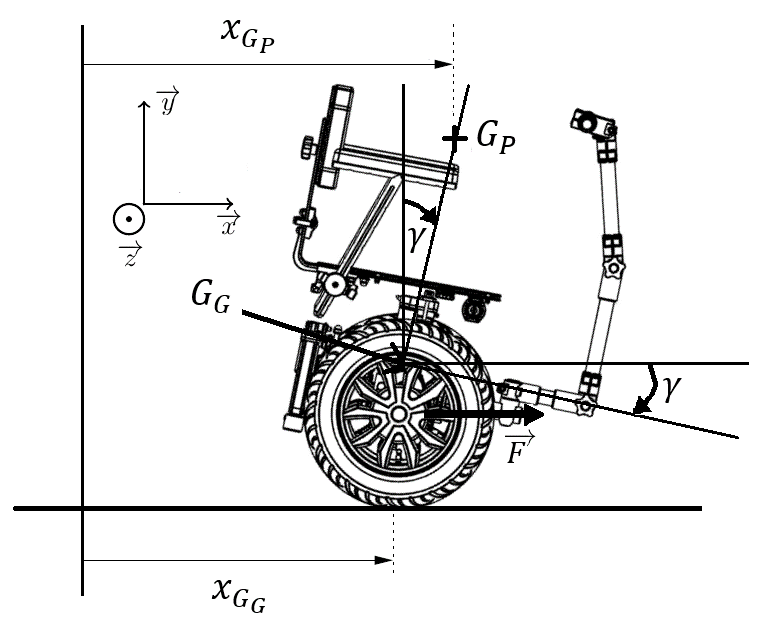
\includegraphics[width=\linewidth]{img/fig16}
\caption{\label{fig16}Paramétrage du modèle}
\end{minipage}
\end{figure}

\begin{itemize}
\item Le fauteuil se déplace en ligne droite, sur une route horizontale. Le passager est légèrement incliné vers l'avant et son centre de masse est décalé d'un angle $\gamma$ par rapport à la verticale. Cet angle est mesuré par la présence d'un accéléromètre et d'un gyromètre installés dans la plateforme du GUS. L'accéléromètre, principalement utilisé en
inclinomètre, permet de déterminer la valeur de l'angle $\gamma$, alors que le gyromètre permet de déterminer la vitesse de variation de cet angle,
\item L'angle $\gamma$, angle entre la verticale et la position de $G_P$ est considéré comme suffisamment petit pour admettre la simplification aux petits angles : $\sin(\gamma) \simeq \gamma$. Cette hypothèse tout à
fait réaliste en pratique permet d'assurer que le passager du fauteuil n'a pas, de son coté, à rechercher son équilibre,
\item On pose $\ell$, distance entre la position du centre de gravité $G_G$ du GUS et $G_P$, la position du centre de gravité du passager,
\item La force $\vec{F}$ permet de maintenir le fauteuil en équilibre.
\end{itemize}

\begin{figure}[ht!]
\begin{minipage}{0.5\linewidth}
\subsection{Fonction de transfert en boucle ouverte}

Avec cet ensemble d'hypothèses, le système se comporte alors comme un simple pendule inversé. On obtient ainsi la fonction de transfert en boucle ouverte dans laquelle, on pose :

\end{minipage}\hfill
\begin{minipage}{0.45\linewidth}
\centering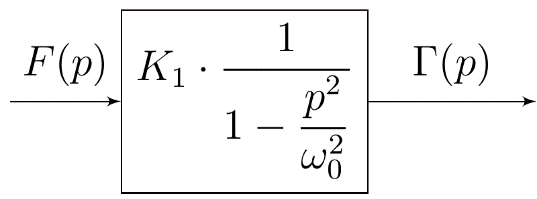
\includegraphics[width=\linewidth]{img/fig17}
\caption{\label{fig17}Fonction de transfert en boucle ouverte du fauteuil et de son passager}
\end{minipage}
\end{figure}

$$H_1(p) = \frac{\Gamma(p)}{F(p)} = \frac{K_1}{(1-\frac{p^2}{\omega_0^2})}\ avec\ K_1 = \frac{1}{\left(M_{Gus} + m_{Passager}\right) \cdot g}\ et\ \omega_0 = \sqrt{\frac{(M_{Gus} + m_{Passager}) \cdot g}{M_{Gus} \cdot l}}$$

\textbf{Applications numériques :} $K_1 = 0,728 \cdot 10^{-3}$ $s^2 \cdot kg^{-1} \cdot m^{-1}$ et $\omega_0 = 6,77$ $rad \cdot s^{-1}$

~\

On rappelle qu'un système est stable si toutes les racines du dénominateur de sa fonction de transfert (aussi appelées pôles) sont à partie réelle négative.

\question{Après avoir déterminé les deux racines du dénominateur, indiquer, en le justifiant, si le système constitué du GUS et de son passager est stable en l'absence d'asservissement. Pour quelle(s) raison(s) pouvions-nous prévoir un tel résultat ?}

~\

\begin{figure}[ht!]
\begin{minipage}{0.5\linewidth}
On place désormais la fonction de transfert $H_1(p)$ sous la forme :

$$H_1(p) = \frac{\Gamma(p)}{F(p)} = \frac{K_1}{(1-\tau \cdot p) \cdot (1+\tau \cdot p)}\ avec\ \tau = \frac{1}{\omega_0}$$
\end{minipage}\hfill
\begin{minipage}{0.45\linewidth}
\centering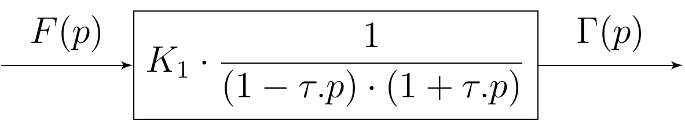
\includegraphics[width=\linewidth]{img/fig18}
\caption{\label{fig18}Fonction de transfert en boucle ouverte du fauteuil et de son passager}
\end{minipage}
\end{figure}

\newpage

\subsection{Stabilisation du système – Fonction de transfert en boucle fermée}

Le correcteur retenu pour stabiliser le système est un correcteur $C(p)$, dit correcteur à avance de
phase. La fonction de transfert de ce type de correcteur est :

$$C(p) = K_C \cdot \frac{1 + a \cdot \tau_c \cdot p}{1 + \tau_c \cdot p}
\ avec\ a = 10.$$

Le système corrigé se présente désormais sous la forme suivante (figure \ref{fig19}) :
\begin{figure}[ht!]
\centering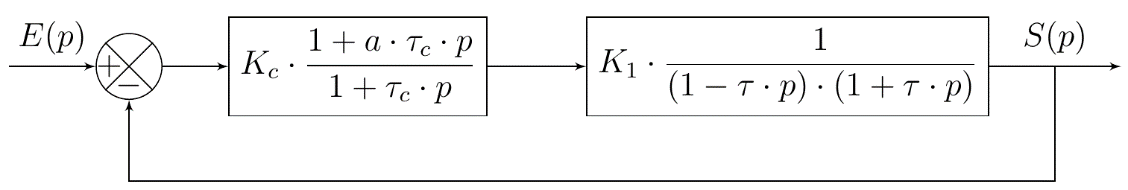
\includegraphics[width=\linewidth]{img/fig19}
\caption{\label{fig19}Boucle fermée du système corrigé}
\end{figure}

On pose :
\begin{itemize}
 \item $FTBO(p) = C(p) \cdot H_1(p)$,
 \item$a \cdot \tau_c = \tau.$
\end{itemize}

On définit la boucle fermée $FTBF(p)$ par le rapport de $S(p)$ par $E(p)$ soit :

$$FTBF(p) = \frac{S(p)}{E(p)}$$

\question{Déterminer l'expression de la boucle fermée $FTBF(p)$ en fonction des paramètres $\tau$, $a$, $K_1$ et $K_C$. Mettre cette expression sous la forme suivante :

$$\frac{S(p)}{E(p)} = \frac{K_2}{a_0 + a_1 \cdot p + a_2 \cdot p^2}\ 
avec\ a_0 = (1 + K_1 \cdot K_c).$$

Identifier les paramètres $K_2$, $a_1$ et $a_2$ de la fonction de transfert en boucle fermée $FTBF(p)$.}

~\

On rappelle qu'un système du second ordre est stable si tous les coefficients du dénominateur de sa fonction de transfert sont de même signe.

\question{Justifier que les signes des coefficients  $a_0$, $a_1$ et $a_2$ doivent être les mêmes ? Quel doit être alors le signe du coefficient $a_0$ pour stabiliser le système ? En déduire l'expression de $K_c$ en fonction de $K_1$ et faire l'application numérique.}

\subsection{Étude du système corrigé}

On pose désormais $K_c = -3000$.

Avec cette valeur de $K_c$, la fonction de transfert du système corrigé en boucle fermée $FTBF(p)$
devient :

$$\frac{S(p)}{E(p)} = FTBF(p) = \frac{2,25}{1,125 + 0,125 \cdot p + 2,25 \cdot 10^{-3} \cdot p^2} = \frac{K}{1 + 2 \cdot z \cdot \frac{p}{\omega_n} + \frac{p^2}{\omega_n^2}}$$

\question{Identifier les paramètres significatifs $K$, $z$ et $\omega_n$ et réaliser les applications numériques.}

~\

Pour valider le fonctionnement global, on réalise, en simulation un essai de réponse du système corrigé à un échelon unitaire (échelon d'Heaviside). On pose alors :

$$E(p) = \frac{1}{p}$$

Le résultat de cet essai est présenté sur la figure 20.

\begin{figure}[ht!]
\centering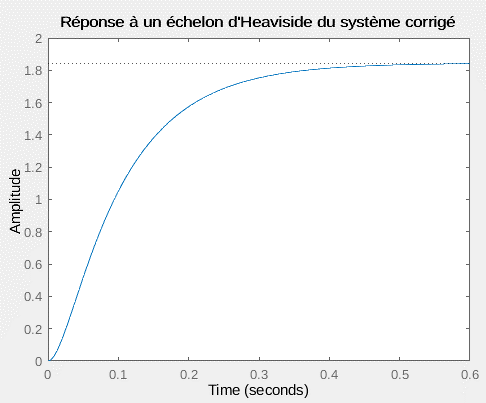
\includegraphics[width=0.8\linewidth]{img/fig20}
\caption{\label{fig20}Réponse du système corrigé en boucle
fermée à une entrée de type échelon d'Heaviside}
\end{figure}


\question{Compte tenu de la valeur numérique de $z$, justifier que la réponse du système à cet échelon d'Heaviside ne présente pas de dépassement. Un essai en réel avec un passager conduirait-t-il à un comportement oscillatoire du fauteuil et de son passager ?}

\question{A l'aide du théorème de votre choix, justifier la valeur de la sortie quand le système est stabilisé. Déterminer la valeur du temps de réponse à 5\%, $tr_{5\%}$ et conclure sur la dynamique globale du système corrigé.}

\subsection{Conclusion}

\question{Conclure quant à la stabilité du système corrigé.}

\section{Identification des versions du GUS}

\paragraph{Objectif :} Réalisation des exigences 1.7 et 1.7.1 : Identifier chaque version du GUS et in fine chaque choix de conception par un système de repérage rapide à mettre en \oe uvre et simple à décoder.

\subsection{Présentation générale}

Les étapes successives de développement du GUS ont nécessité une identification simple des modèles. Un code-barres de type EAN8, placé de manière adéquate, permet à l'opérateur d'identifier sans ambiguïté chaque modèle du GUS grâce à l'interprétation de ce dernier. Une base de données permet de retrouver les choix de conception lors de chaque étape de recherche et développement.

\subsection{Création des codes-barres de type EAN8}

Un code-barres de type EAN8 se compose de sept données numériques utiles suivies d'une clé de contrôle sur un seul chiffre. Dans le cas du GUS, les sept données utiles du code-barres sont générées de la manière suivante :

\begin{itemize}
\item les quatre premiers chiffres servent à identifier l'année de conception. Ce nombre est strictement supérieur à 2013 ;
\item les deux suivants sont réservés au mois de conception. Ce nombre est compris entre 01 et 12 inclus ;
\item celui d'après est réservé au modèle dans le mois en supposant
que plusieurs prototypes existent dans le mois considéré. Ce
nombre est supérieur ou égal à 1 et ne dépassera jamais 9.
\end{itemize}

\textbf{Exemple :}
Le premier prototype date de 2014.
Il est sorti au mois de Mai (05).
Il est le premier et le seul développé lors de ce mois.

\newpage

Ainsi le code-barres EAN 8 de valeur 2014051, associé à sa clé de contrôle de valeur 9, identifie de manière unique le premier et seul prototype sorti au mois de Mai 2014.

\subsection{Création du code de contrôle}

Le code de contrôle est nécessaire lors des étapes de lecture pour s'assurer que cette dernière se fait sans erreur. Sa réalisation dépend d'une procédure algorithmique.

\question{A partir du document technique DT7, justifier que la clé de contrôle correspondant au premier prototype est bien égale à la valeur 9.}

\question{Citer au moins un autre mode de contrôle classiquement utilisé pour vérifier les échanges dans les transmissions de données.}

\subsection{Codage de la version du GUS}

\question{A partir du document technique DT7, indiquer quel est le nombre de bits, présents dans un code EAN 8 et en déduire le nombre de bandes de largeur élémentaire présentes dans chaque code EAN 8.}

\question{Pour un même chiffre, indiquer quelle est l'opération logique nécessaire pour passer de la représentation binaire dans la colonne nommée \textbf{Gauche} du tableau, correspondant à la première partie du code, à sa représentation dans la colonne nommée \textbf{Droite} du tableau, correspondant à la seconde partie du code.}

~\

On appelle distance de Hamming $d_{A \leftrightarrow B}$ entre deux éléments $A$ et $B$ d'un code binaire constitués chacun de $n$ bits, le nombre de bits qui change d'état entre ces deux éléments pour un rang $i$
donné.

Cette distance peut se calculer de la manière suivante :

$$d_{A \leftrightarrow B} = \sum_{i=0}^{n-1} (a_i \oplus b_i) = \sum_{i=0}^{n-1} (a_i \cdot \overline{b_i} + \overline{a_i} \cdot b_i)$$

avec $A = [a_{n-1} \ldots a_0]$ et $B = [b_{n-1} \ldots b_0]$

~\

On s'intéresse uniquement à la colonne nommée \textbf{Gauche} du tableau du document technique DT7. Dans cette colonne, le codage du chiffre 0, pris comme élément de référence, s'écrit $(0001101)_2$.

On appelle $d_{(0 \leftrightarrow \{1,2,3,4,5\})_{min}}$, la distance de Hamming minimale entre les distances $d_{0 \leftrightarrow i}$ avec
$i \in \llbracket 1,5 \rrbracket$.

\question{Pour la colonne nommée \textbf{Gauche} du document technique DT7, compléter le tableau du document réponse, représentant les distances de Hamming $d_{0 \leftrightarrow i}$ entre le codage du chiffre 0 et le codage des chiffres de 1 à 5. Quelle est la distance minimale
$d_{(0 \leftrightarrow \{1,2,3,4,5\})_{min}}$ obtenue ?}

~\

On montre que la valeur de la distance $d_{(0 \leftrightarrow \{1,2,3,4,5\})_{min}}$, déterminée à la question précédente
correspond à la distance minimale entre tous les codages pour la colonne nommée \textbf{Gauche} quel que soit le chiffre pris comme élément de référence.

\question{Cette distance est-elle identique pour la représentation des chiffres de la colonne nommé \textbf{Droite} ?}

~\

Le code barre du document technique DT8 est collé sur un des derniers prototypes de GUS avant son début de commercialisation.

\question{Sur le document réponse, compléter le tableau et déchiffrer le code EAN 8, présent sur le document technique DT8, en indiquant en particulier l'année et le numéro de prototype de la version du GUS identifiés par ce code-barres.}

\section{Synthèse sur l'étude – Conclusion générale}

\question{En reprenant les différents points abordés, énoncer en quelques lignes une synthèse des grandes étapes de l'étude du GUS et les limites des modélisations proposées. Quels sont les points qui restent à améliorer dans cette étude ?}

\begin{figure}[ht!]
\begin{center}
 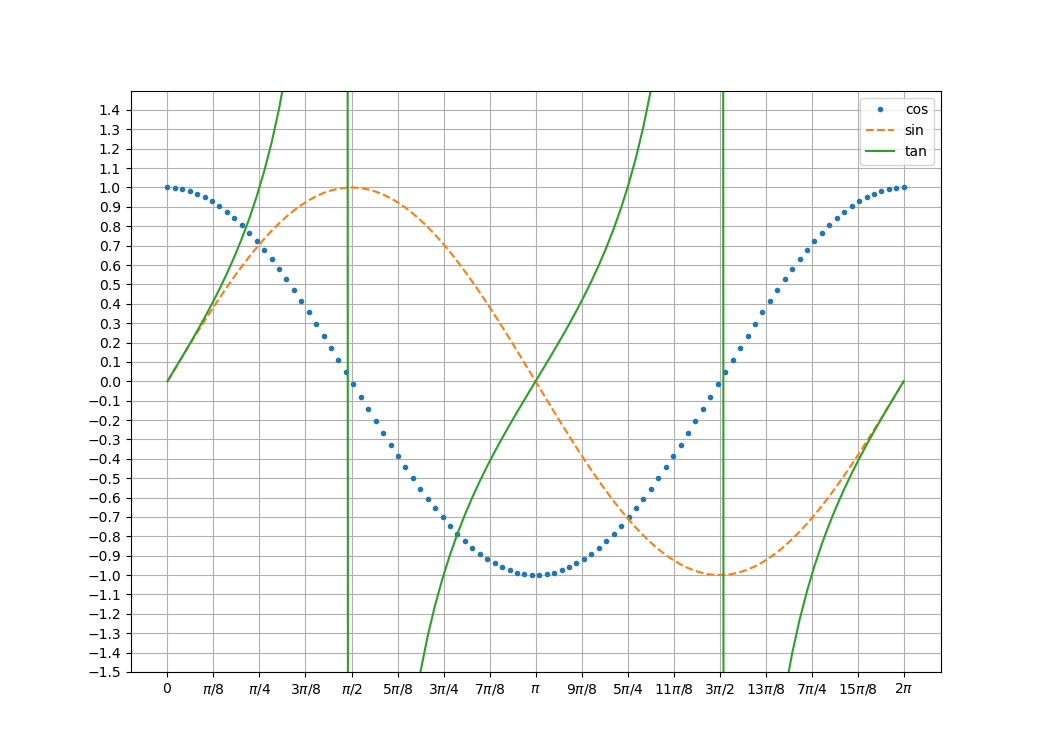
\includegraphics[width=0.7\linewidth]{img/cossintan}
\end{center}
\caption{\label{cossintan}Tracé des fonctions cos, sin et tan}
\end{figure}

\finsujet

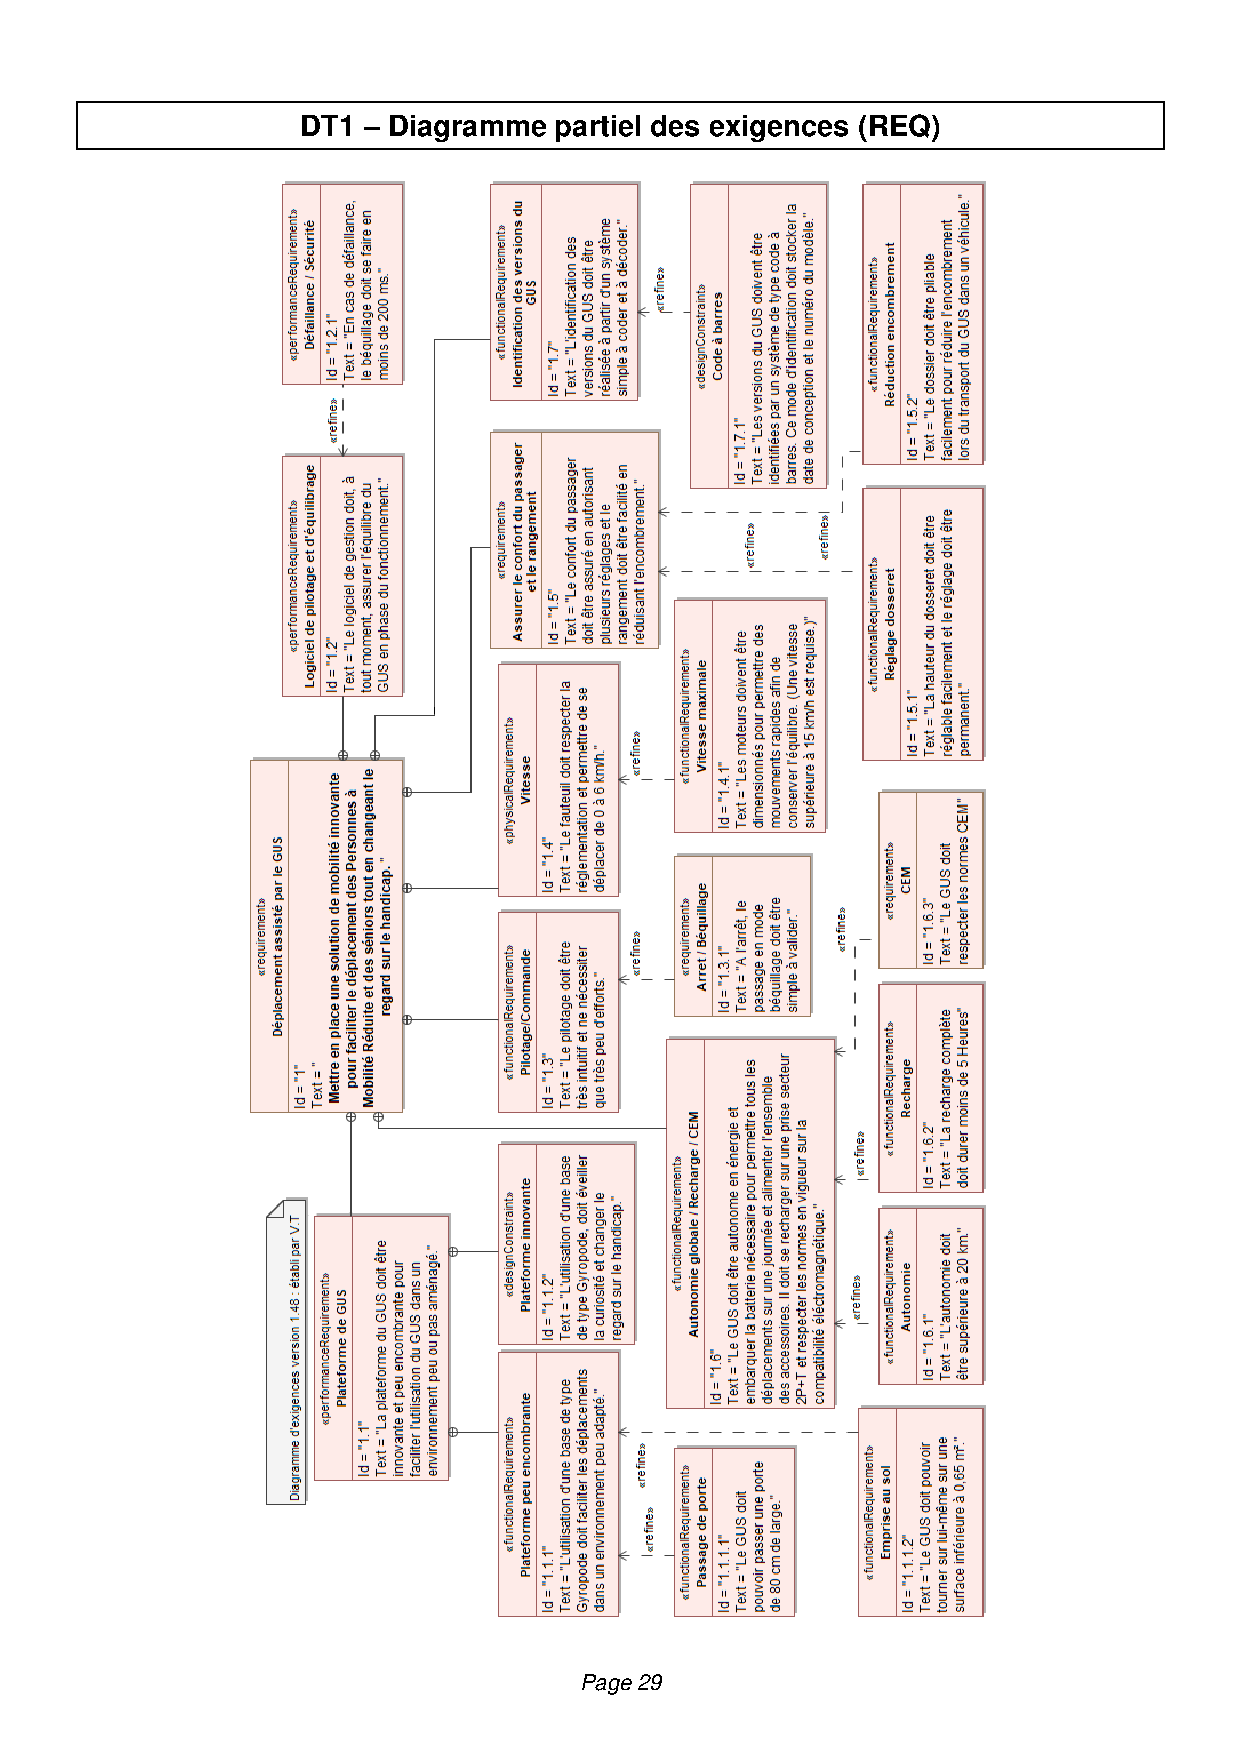
\includepdf[pages=1-10]{img/annexes.pdf}

\debutcor

%1
\reponse{2}{}{
On peut lire sur le document DT1 les informations suivantes :
\begin{itemize}
  \item Exigence 1.6.1 : 20 km d'autonomie.
  \item Exigence 1.4 : Vitesse maximale de 6 km/h.
  \item Exigence 1.1.1.2 : Une surface nécessaire inférieure à 0,65 m².
\end{itemize}

Un déplacement de 20 km par jour est assez important, donc l'autonomie journalière est très largement satisfaisante.}

%2
\reponse{1}{\begin{center}
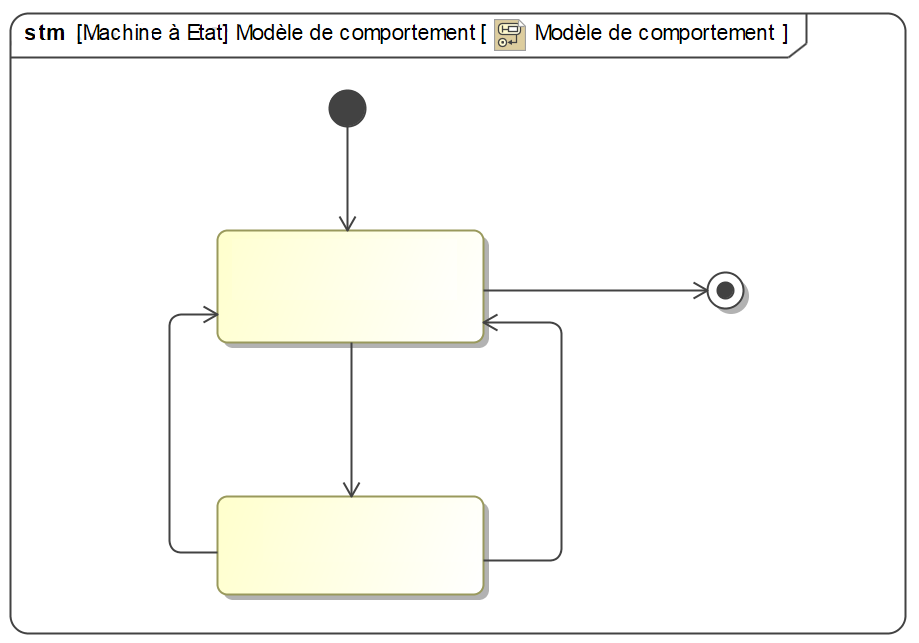
\includegraphics[width=0.5\linewidth]{img/dr01}
\end{center}
}{
Il suffit de compléter les états manquants et les transitions manquantes à partir de la description fonctionnelle proposée.
On peut accepter une seule flèche avec un OU dans les deux conditions : CAB + CMB

\begin{center}
\def\svgwidth{0.6\linewidth}
  \input{img/dr01_cor.pdf_tex}
\end{center}
}

%3
\reponse{1}{\begin{center}
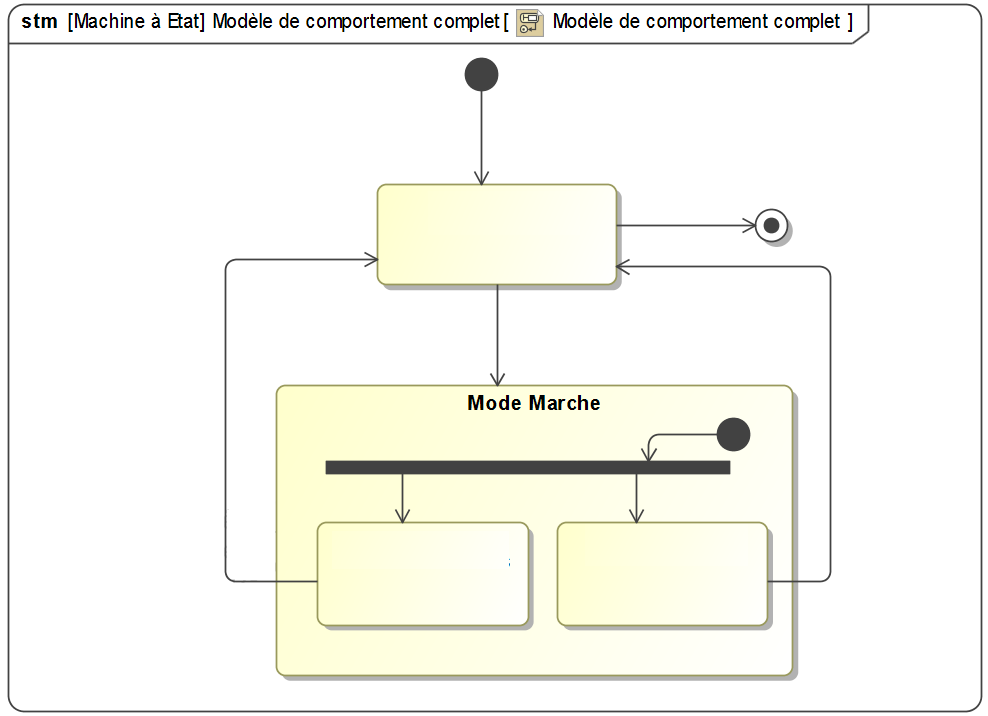
\includegraphics[width=0.5\linewidth]{img/dr02}
\end{center}}{
Il suffit de compléter les états manquants et les transitions manquantes à partir de la description fonctionnelle proposée.

\begin{center}
\def\svgwidth{0.6\linewidth}
  \input{img/dr02_cor.pdf_tex}
\end{center}
}

%4
\reponse{2}{}{
Le béquillage est automatique et se fait en moins de 200 ms. Les exigences 1.2 et 1.2.1 sont donc respectées.}

%5
\reponse{0}{\begin{center}
\begin{tabular}{|m{6cm}|m{6cm}|m{5cm}|}
\hline
\textbf{De} & \textbf{Vers} & \textbf{Type de flux}\\
\hline
: Batterie & : Hacheur quatre quadrants [2] & \\
\hline
: Hacheur quatre quadrants [2] & : MotoRéducteur CC [2] & \\
\hline
: MotoRéducteur CC [2] & : Roue [2] & \\
\hline
: Roue [2] & : Route & \\
\hline
\end{tabular}
\end{center}

\begin{center}
\begin{tabular}{|m{6cm}|m{6cm}|m{5cm}|}
\hline
\textbf{De} & \textbf{Vers} & \textbf{Type de flux}\\
\hline
: MotoRéducteur CC [2] (entrée du bloc) & : MCC & \\
\hline
: MCC & : Réducteur & \\
\hline
: Réducteur & : MotoRéducteur CC [2] (sortie du bloc) & \\
\hline
\end{tabular}
\end{center}}{
\begin{center}
\begin{tabular}{|m{5cm}|m{5cm}|m{5cm}|}
\hline
\textbf{De} & \textbf{Vers} & \textbf{Type de flux}\\
\hline
: Batterie & : Hacheur quatre quadrants [2] & Flux énergie électrique\\
\hline
: Hacheur quatre quadrants [2] & : MotoRéducteur CC [2] & Flux énergie électrique\\
\hline
: MotoRéducteur CC [2] & : Roue [2] & Flux énergie mécanique de rotation\\
\hline
: Roue [2] & : Route & Flux énergie mécanique de translation\\
\hline
\end{tabular}
\end{center}

\begin{center}
\begin{tabular}{|m{5cm}|m{5cm}|m{5cm}|}
\hline
\textbf{De} & \textbf{Vers} & \textbf{Type de flux}\\
\hline
: MotoRéducteur CC [2] (entrée du bloc) & : MCC & Flux énergie électrique\\
\hline
: MCC & : Réducteur & Flux énergie mécanique de rotation\\
\hline
: Réducteur & : MotoRéducteur CC [2] (sortie du bloc) & Flux énergie mécanique de rotation\\
\hline
\end{tabular}
\end{center}
}

%6
\reponse{5}{}{
Sur la documentation du moteur, on peut lire que sa vitesse de sortie du moto-réducteur en charge est de 200 rpm, soit 200 tours par minute. On obtient donc une vitesse de 
$$\omega = 200 \cdot \frac{2\pi}{60} \approx 20 rad\cdot s^{-1}$$

Le diamètre de la roue est de 42 cm, soit 
$$V = \frac{D_R}{2} \cdot \omega = 0,21 \cdot 20 = 4,2 m\cdot s^{-1}$$

Cette vitesse correspond à 
$$V = 4,2 \cdot \frac{3600}{1000} = 15,12 km\cdot h^{-1}$$

Donc, l'exigence 1.4.1 est satisfaite.}

%7
\reponse{4}{}{La puissance à vide vaut $P_{vide} = U_0 \cdot I_0$. L'énoncé dit que 
$$P_{vide} = U_0 \cdot I_0 = P_{Joule} + P_{Pertes\ collectives} = R \cdot I_0^2 + C_p \cdot \Omega_{vide}$$

donc
$$C_p = \frac{U_0 \cdot I_0 - R \cdot I_0^2}{N_{vide}} \cdot \frac{60}{2\pi} = \frac{36 \cdot 3,3 - 0,4 \cdot 3,3^2}{250} \cdot \frac{60}{2\pi} = 4,37 N\dot m$$
}


%8
\reponse{6}{}{
La puissance nominale est de 500 W en charge avec une vitesse de 200 rpm (tours par minute). On a donc:

$$P_u = C_{nom} \cdot \Omega_{nom} \Rightarrow C_{nom} = \frac{P_u}{\Omega_{nom}} = \frac{P_u}{N_{nom}} \cdot \frac{60}{2\pi} = \frac{500}{200} \cdot \frac{60}{2\pi} \approx 25 N\cdot m$$

Le couple maximal est : 
$$C_{max} = \frac{P_{max}}{\Omega_{nom}} = \frac{P_{max}}{N_{nom}} \cdot \frac{60}{2\pi} = \frac{1000}{200} \cdot \frac{60}{2\pi} \approx 50 N\cdot m$$

Le rendement nominal est :
$$\eta = \frac{P_u}{P_{abs}} = \frac{P_u}{U_0 \cdot I_0} = \frac{500}{36 \cdot 17}= \frac{500}{612} \approx 83,3\%$$

Le rendement nominal est assez bon, surtout avec le réducteur à engrenages.}

%9
\reponse{6}{}{
Il faut prendre en compte le réduction.

$$\Omega_{M_{vide}} = R_{red} \cdot N_{vide} \cdot \frac{2\pi}{60} = 17 \cdot 250 \cdot \frac{2\pi}{60} \approx 425 \text{ rad}\cdot\text{s}^{-1}
$$

On peut alors en déduire le coefficient $K_E$ et on obtient 
$$E = K_E \cdot \Omega_M \Rightarrow K_E = \frac{36}{425}\approx \frac{7}{85} \approx 0,08 V\cdot rad\cdot s^{-1}\ ou\ V\cdot s^{-1}$$
}

%10
\reponse{6}{}{
$$\sin(\delta) = \frac{C_{Total}}{m_{passager} \cdot g \cdot \ell} \Rightarrow \delta = \arcsin\left(\frac{C_{Total}}{m_{passager} \cdot g \cdot \ell}\right)$$

Par application numérique, on a :
$$\delta_{min} = \arcsin\left(\frac{C_{Total}}{\ell \cdot m_{passager\ max} \cdot g}\right) = \arcsin\left(\frac{2 \cdot 48}{0,5 \cdot 100 \cdot 9,81}\right) = 11,5\textdegree$$

La valeur de cet angle augmente si la masse du passager diminue, c'est donc le pire des cas.

Le couple est compatible avec un angle de $\delta_{min}$, il faut que le béquillage entre en jeu pour un angle plus petit que celui-ci.}

%11
\reponse{2}{\begin{center}
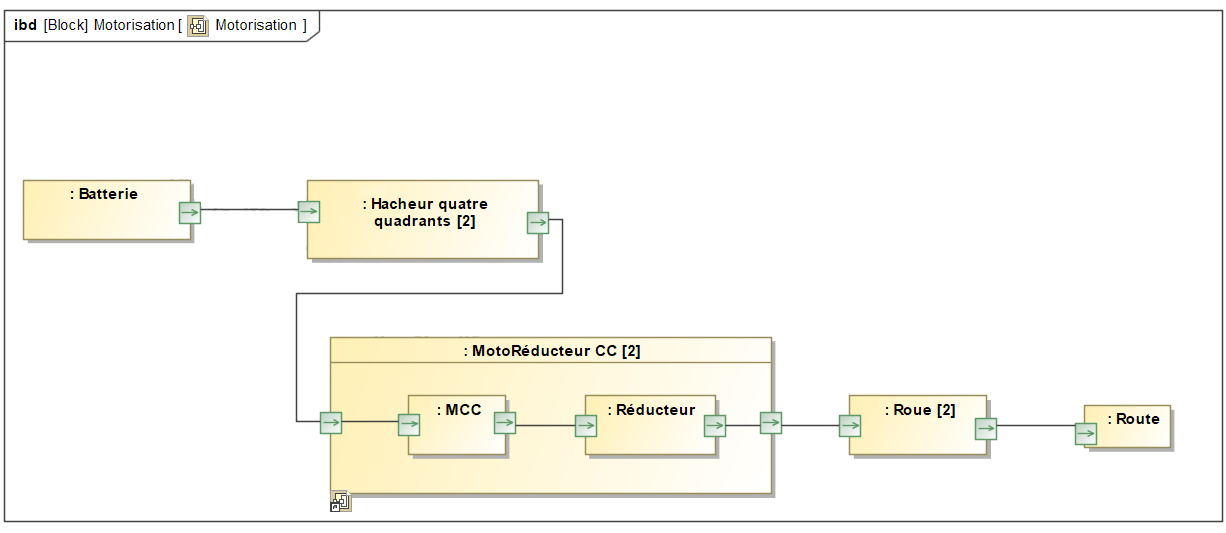
\includegraphics[width=0.9\linewidth]{img/dr03}
\end{center}}{
Flux d'information entre la carte de commande et le hacheur (4 transistors par hacheur et deux hacheurs, il y a 8 informations en parallèle).
\begin{center}
\def\svgwidth{0.6\linewidth}
  \input{img/dr03_cor.pdf_tex}
\end{center}}

%12
\reponse{3}{}{
Il faut 4 quadrants car le moteur fonctionne dans les deux sens et puisse fonctionner en générateur. Il faut donc un 4 quadrants.

Il faut trois segments pour l'interrupteur $K_i$. Il faut ainsi que chaque interrupteur soit bidirectionnel en courant et unidirectionnel en tension.}

%13
\reponse{3}{}{
Le DT indique pour l'interrupteur une tension max de 55 V. La tension maximale de la batterie est de 36 V. Le coefficient de sécurité est de $\frac{36}{55} \approx 0,7$.

Le courant max est de 34 A, le courant max dans le transistor est de 169 A, le coefficient de sécurité est de $\frac{34}{169} = 0,2$. Le choix de l'interrupteur de commande est donc tout à fait valide.}

%14
\reponse{1}{
\begin{center}
\begin{tabular}{|c|c|c|c|c|c|c|c|c|c|c|c|}
\hline
$K_1$ & $K_2$ & $K_3$ & $K_4$ & $T_1$ & $D_1$ & $T_2$ & $D_2$ & $T_3$ & $D_3$ & $T_4$ & $D_4$ \\
\hline
 & & & & & & & & & & &  \\
\hline
\end{tabular}
\end{center}
}{
\begin{center}
\begin{tabular}{|c|c|c|c|c|c|c|c|c|c|c|c|}
\hline
$K_1$ & $K_2$ & $K_3$ & $K_4$ & $T_1$ & $D_1$ & $T_2$ & $D_2$ & $T_3$ & $D_3$ & $T_4$ & $D_4$ \\
\hline
Ac & Ac & In & In & Ac & In & In & Ac & In & In & In & In  \\
\hline
\end{tabular}
\end{center}

On reconnaît ici un hacheur série.}

%15
\reponse{1}{}{
$\langle U_m \rangle = \alpha \cdot V_{bat}$.
}


%16
\reponse{2}{}{
Tous les mouvements se font dans le plan et les efforts sont symétriques par rapport à ce plan, on peut donc utiliser cette modélisation.}

%17
\reponse{3}{}{$\tan \theta = \frac{d_v}{d_h}$ soit $\theta = \arctan \frac{d_v}{d_h}$

Par application numérique avec une pente à 10\%, on a $\theta = \arctan \frac{1}{10} = \frac{1}{4}\cdot\frac{\pi}{8}\approx 0,1$ rad}

%18
\reponse{3}{}{
$\theta$ est petit donc $\sin(\theta)=\tan(\theta)$, donc

$F_{RT} = M \cdot g \cdot \sin(\theta) = 160 \cdot 9,81 \cdot \dfrac{1}{10} = 156,8N$}

%19
\reponse{3}{}{
$\theta$ est petit donc $\cos(\theta)=1$, donc

On obtient directement $F_{Roul} = -M \cdot g \cdot C_{rr} \cdot \cos(\theta) = -160 \cdot 9,81 \cdot 0,02 = -31,36$ N

$F_{Roul}$ représente 20\% de $F_{RT}$, il ne peut pas être négligée.}

%20
\reponse{5}{}{
On a:
$d_g = R_{int} \cdot \varphi$ et $d_d = R_{ext} \cdot \varphi = (R_{int} + dl) \cdot \varphi$ 

$d_d - d_g = (R_{int} + dl) \cdot \varphi - R_{int} \cdot \varphi = d_{\ell} \cdot \varphi$
donc $\varphi = \frac{d_d - d_g}{d_{\ell}} = \frac{13,15 - 11,52}{0,63} =\frac{1,63}{0,63}=\frac{1}{\frac{2}{3}}+1 = 2,5$ rad}

%21
\reponse{5}{}{
$R=\dfrac{R_{int}+R_{ext}}{2}$

$R=\dfrac{d_g+d_d}{2\cdot\varphi}$

Donc, $R = \frac{d_{\ell}}{2} \cdot \frac{d_d + d_g}{d_d - d_g} = \frac{0,63}{2} \cdot \frac{24,67}{1,63} = 24,67\cdot 0,2 \approx 5$ m

On obtient donc $d_p = R \cdot \varphi = 5 \cdot 2,59 = 13$ m.}

%22
\reponse{2}{\begin{center}
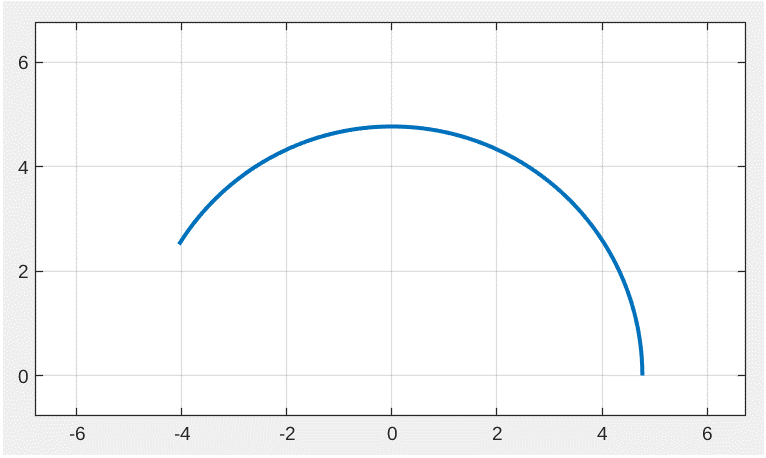
\includegraphics[width=0.9\linewidth]{img/dr04}
\end{center}}{
\begin{center}
\def\svgwidth{0.6\linewidth}
  \input{img/dr04_cor.pdf_tex}
\end{center}}

%23
\reponse{4}{}{
\begin{center}
\def\svgwidth{0.6\linewidth}
  \input{img/dr05_cor.pdf_tex}
\end{center}}

%24
\reponse{8}{}{
Par l'approche cinématique, on peut écrire les deux torseurs suivants:
$$\left\{V_{1/0}^{1}\right\} = \left\{
\begin{array}{cc}
0 & 0\\
0 & 0\\
\Omega_{1/0}^{1} &V_{A \in 1/0}^{1}
\end{array}
\right\}_A\ et\ \left\{V_{1/0}^{2}\right\} = \left\{
\begin{array}{cc}
0 & 0\\
0 & 0\\
\Omega_{1/0}^{2} &V_{B \in 1/0}^{2}
\end{array}
\right\}_B$$

On déplace le premier torseur $\left\{V_{1/0}^{1}\right\}$ au point B, on a:
$$\overrightarrow{V_{B \in 1/0}^{1}} = \overrightarrow{V_{A \in 1/0}^{1}} + \overrightarrow{BA} \wedge \overrightarrow{\Omega}_{1/0}^{1} = V_{A,z}^{1} \cdot \vec{z} - L \cdot \vec{y} \wedge \omega_z^{1} \cdot \vec{z} = V_{A,z}^{1} \cdot \vec{z} - L \cdot \omega_z^{1} \cdot \vec{x}$$

Soit,
\begin{eqnarray}
\vec{x}: \omega_x^{eq} = 0 = 0 \nonumber \\
\vec{y}: \omega_y^{eq} = 0 = 0 \nonumber \\
\vec{z}: \omega_z^{eq} = \omega_z^{1} = \omega_z^{2} \nonumber \\
\vec{x}: V_{B,x}^{eq} = -L \cdot \omega_z^{1} = 0  \nonumber \\
\vec{y}: V_{B,y}^{eq} = 0 = 0  \nonumber \\
\vec{z}: V_{B,z}^{eq} = V_{A,z}^{1} = V_{B,z}^{2} \nonumber
\end{eqnarray}

$$\left\{V_{1/0}^{eq}\right\} = \left\{
\begin{array}{cc}
0 & 0\\
0 & 0\\
0 &V_{B \in 1/0}^{2}
\end{array}
\right\}_B$$

La liaison équivalente est donc une glissière de direction $\vec{z}$.}

%25
\reponse{5}{}{
Méthode cinématique: Soit $h =E_c-I_c+m =6-4+1=3$

Méthode statique: $h = N_s - r_s=8-6\cdot(2-1)+1=3$

Il faut donc les deux conditions géométriques suivantes:
\begin{itemize}
    \item Les deux axes $(A,\vec{z})$ et $(B,\vec{z})$ sont parallèles (angles $\theta_y$ et $\theta_z$),
    \item même entraxe $AB$ (distance $y$).
\end{itemize}}

%26
\reponse{5}{}{ La translation est supprimée par serrage des écrous à volant. L'exigence 1.5.1 est donc réalisée.}

%27
\reponse{5}{}{En intégrant sur toute la surface, on a :

$$\overrightarrow{R_{2 \rightarrow 1}} = \int (-p_n \cdot \vec{z} + p_t \cdot \vec{v}) \cdot ds= \int (-p_n \cdot \vec{z} + p_t \cdot (-\sin(\theta) \cdot \vec{x} + \cos(\theta) \cdot \vec{y})) \cdot r \cdot dr \cdot d\theta$$

$$\overrightarrow{R_{2 \rightarrow 1}} = \int_{\theta=0}^{\theta=2\pi} (-p_n \cdot \vec{z} + p_t \cdot (-\sin(\theta) \cdot \vec{x} + \cos(\theta) \cdot \vec{y})) \cdot d\theta \int_{r=r_{int}}^{r=r_{ext}} r \cdot dr$$

$$\vec{R}_{2 \rightarrow 1} = -p_n \cdot \vec{z} \cdot 2 \cdot \pi \cdot \frac{(r_{ext}^2 - r_{int}^2)}{2} = -p_n \cdot \pi \cdot (r_{ext}^2 - r_{int}^2) \cdot \vec{z}$$

On a :$\overrightarrow{R_{2 \rightarrow 1}} = -F \cdot \vec{z}$ soit $-p_n \cdot \pi \cdot (r_{ext}^2 - r_{int}^2) \cdot \vec{z} = -F \cdot \vec{z}$

Ainsi, $p_n = \frac{F}{\pi \cdot (r_{ext}^2 - r_{int}^2)}$
}

%28
\reponse{6}{}{$$\overrightarrow{M_{O,2\rightarrow1}} = \int \vec{OM} \wedge \overrightarrow{dF_{2\rightarrow1}(M)}= \int r \cdot \vec{u} \wedge (-p_n \cdot \vec{z} + p_t \cdot \vec{v}) \cdot ds = \int r \cdot (p_n \cdot \vec{v} + p_t \cdot \vec{z}) \cdot r \cdot dr \cdot d\theta $$

$$\overrightarrow{M_{O,2\rightarrow1}} = \int_{\theta=0}^{\theta=2\pi} \left(p_n \cdot (-\sin(\theta) \cdot \vec{x} + \cos(\theta) \cdot \vec{y}) + p_t \cdot \vec{z}\right) \cdot d\theta \int_{r=r_{int}}^{r=r_{ext}} r^2 \cdot dr$$

$$\overrightarrow{M_{O,2\rightarrow1}} = p_t \cdot 2 \cdot \pi \cdot \vec{z} \cdot \frac{(r_{ext}^3 - r_{int}^3)}{3} = \frac{2}{3} \cdot \pi \cdot f \cdot p_n \cdot (r_{ext}^3 - r_{int}^3) \cdot \vec{z}$$}

%29
\reponse{3}{}{
$$C_S = \overrightarrow{M_{O,2\rightarrow1}}\cdot\vec{z}=\frac{2}{3} \cdot f \cdot F \cdot \frac{\left(r_{ext}^3 - r_{int}^3\right)}{\left(r_{ext}^2 - r_{int}^2\right)}$$}

%30
\reponse{3}{}{
$$C_{S_{Total}} = 4 \cdot \frac{2}{3} \cdot f \cdot F \cdot \frac{\left(r_{ext}^3 - r_{int}^3\right)}{\left(r_{ext}^2 - r_{int}^2\right)}$$}

%31
\reponse{1}{}{
L'angle maximal de la charnière est de 215°, elle convient pour un angle de 90°. L'exigence de pliage est donc validée.}

%32
\reponse{5}{}{$$H_1(p) = \frac{\Gamma(p)}{F(p)} = \frac{K}{\left(1 - \frac{p}{\omega_0}\right) \left(1 + \frac{p}{\omega_0}\right)}$$

Les deux racines sont donc :
$$p_1 = \omega_0 \text{ et } p_2 = -\omega_0$$

Comme une des racines a une partie réelle positive, cela signifie que le système est instable.}

%33
\reponse{8}{}{
$$FTBO(p) = \frac{K_c\cdot K_1}{\left(1+\tau_c\cdot\right)\cdot \left(1-\tau\cdot p\right)}$$, avec $a \cdot \tau_c = \tau$.

$$\frac{S(p)}{E(p)} = FTBF(p) = \frac{FTBO}{1 + FTBO} = \frac{K_1 \cdot K_c}{\left(1 + \frac{\tau}{a} \cdot p\right) \cdot (1 - \tau \cdot p)} \cdot \frac{1}{1 + \frac{K_1 \cdot K_c}{\left(1 + \frac{\tau}{a} \cdot p\right) \cdot (1 - \tau \cdot p)}}$$

$$\frac{S(p)}{E(p)}= \frac{K_1 \cdot K_c}{\left(1 + \frac{\tau}{a} \cdot p\right) \cdot (1 - \tau \cdot p) + K_1 \cdot K_c}$$

$$\frac{S(p)}{E(p)} = \frac{K_1 \cdot K_c}{(1 + K_1 \cdot K_c) - \tau \cdot \left(1 - \frac{1}{a}\right) \cdot p - \frac{\tau^2}{a} \cdot p^2}$$

On a donc par identification :
\begin{align}
K_2 &= K_1 \cdot K_c \nonumber\\
a_0 &= (1 + K_1 \cdot K_c) \nonumber \\
a_1 &= -\tau \cdot \left(1 - \frac{1}{a}\right)  \nonumber\\
a_2 &= -\frac{\tau^2}{a} \nonumber
\end{align}}

%34
\reponse{5}{}{Les coefficients du dénominateur doivent être identiques afin que les parties réelles des racines du polynôme soient négatives.
$a_1<0$ et $a_2<0$, donc il faut $a_0<0$, soit $1+K_1\cdot K_c<0$, donc $K_c<-\dfrac{1}{K_1}$}

%35
\reponse{5}{}{
On obtient :
$$\frac{S(p)}{E(p)} = \frac{2,25}{1,125 + 0,125 \cdot p + 2,25 \cdot p^2} = \frac{2,25}{1,125 \cdot \left(1 + \frac{0,125}{1,125} \cdot p + \frac{2,25 \cdot 10^{-3}}{1,125} \cdot p^2\right)}$$

\begin{align}
K &= \frac{2,25}{1,125} = 2 \nonumber\\
\omega_n &= \sqrt{\frac{1,184}{2,25 \cdot 10^{-3}}} = 22rad\cdot s^{-1} \nonumber \\
z &= \frac{1}{2} \cdot \frac{0.125}{1,125} \cdot \sqrt{\frac{1,125}{2,25 \cdot 10^{-3}}} = 2\nonumber
\end{align}}

%36
\reponse{5}{}{
$z>1$ donc il ne peut pas y avoir de dépassement. Il ne devrait donc pas y avoir de comportement oscillatoire pour le passager sur le fauteuil.}

%37
\reponse{5}{}{D'après le théorème de la valeur finale, on a :
\begin{align}
\lim_{t \to \infty} s(t) &= \lim_{p \to 0} p \cdot S(p) \nonumber\\
&= \lim_{p \to 0} p \cdot FTBF(p) \cdot E(p) \nonumber\\
&= \lim_{p \to 0} p \cdot FTBF(p) \cdot E(p) \text{ avec } E(p) = \frac{1}{p} \nonumber\\
\lim_{t \to \infty} s(t) &= \lim_{p \to 0} p \cdot \frac{2,25}{1,125 \cdot \left(1 + \frac{0,125}{1,125} \cdot p + \frac{2,25 \cdot 10^{-3}}{1,125} \cdot p^2\right)} \cdot \frac{1}{p} \nonumber\\
&= \frac{2,125}{1,125} = 2\nonumber
\end{align}

On lit le temps de réponse : $s(t) = 0,95 \cdot 1,85 \simeq 1,75$ donc $tr_{5\%} \simeq 0,3$ s.

La dynamique globale du système est donc acceptable.}

%38
\reponse{5}{}{
Grace au correcteur à avance de phase et à la valeur du gain $K_c$ le système est stable et rapide, il répond donc au cahier des charges.}

%39
\reponse{4}{}{
Le code est 2014 05 1
\begin{center}
\begin{tabular}{|c|c|c|c|c|c|c|c|}
\hline
Chiffre & 2 & 0 & 1 & 4 & 0 & 5 & 1  \\
\hline
Poids & 3 & 1 & 3 & 1 & 3 & 1 & 3 \\
\hline
      & 6 & 0 & 3 & 4 & 0 & 5 & 3 \\
\hline
\end{tabular}
\end{center}

$6+0+3+4+0+5+3 = 21$

$21\%10 = 1$

$10-1 = 9$

La clé de contrôle est bien 9.}

%40
\reponse{2}{}{On peut citer les systèmes avec test de parité comme le Code de Hamming.}

%41
\reponse{4}{}{Il faut :
\begin{itemize}
 \item 3 bits de garde pour le début,
 \item 4 chiffres codés en 7 bits,
 \item 5 bits de zone de garde centrale,
 \item 4 chiffres codés en 7 bits,
 \item 3 bits de garde pour la fin.
\end{itemize}

Cela fait un total de $3+4*7+5+4*7+3=67bits$. Il faut donc 67 bandes.}

%42
\reponse{5}{}{Un $1$ devient un $0$ et un $0$ devient un $1$, c'est donc un complément à un.}

%43
\reponse{5}{\begin{center}
\begin{tabular}{|c|c|c|c|c|c|}
\hline
Distance de Hamming $d_{0 \leftrightarrow i}$ & $d_{0 \leftrightarrow 1}$ & $d_{0 \leftrightarrow 2}$ & $d_{0 \leftrightarrow 3}$ & $d_{0 \leftrightarrow 4}$ & $d_{0 \leftrightarrow 5}$ \\
\hline
 &  &  &  &  &  \\
\hline
\end{tabular}
\end{center}}{
\begin{center}
\begin{tabular}{|c|c|c|c|c|c|}
\hline
Distance de Hamming $d_{0 \leftrightarrow i}$ & $d_{0 \leftrightarrow 1}$ & $d_{0 \leftrightarrow 2}$ & $d_{0 \leftrightarrow 3}$ & $d_{0 \leftrightarrow 4}$ & $d_{0 \leftrightarrow 5}$ \\
\hline
 & 2 & 4 & 2 & 4 & 4 \\
\hline
\end{tabular}
\end{center}

La distance de Hamming minimale est de 2.}

%44
\reponse{5}{}
{La distance est la même pour la colonne droite (normal, c'est un complément à 1).

Cette solution permet d'éviter les erreurs liées à des valeurs successives trop proches.}

%45
\reponse{5}{\begin{center}
\begin{tabular}{|c|c|c|}
\hline
Champs & Code binaire & Décodage\\
\hline
Zone de garde gauche &  &\\
\hline
Chiffres de gauche & & \\
\hline
Zone de garde centrale &  &  \\
\hline
Chiffres de droite & & \\
\hline
Zone de garde droite & 101 & \\
\hline
\end{tabular}
\end{center}
}{\begin{center}
\begin{tabular}{|c|c|c|}
\hline
Champs & Code binaire & Décodage \\
\hline
Zone de garde gauche & 101 & \\
\hline
Chiffres de gauche & 0010011 0001101 0010011 0011001 & 2021 \\
\hline
Zone de garde centrale & 01010 & \\
\hline
Chiffres de droite & 1110010 1000100 1101100 1011100 & 0724 \\
\hline
Zone de garde droite & 101 & \\
\hline
\end{tabular}
\end{center}

Le prototype a été développé en juillet 2021 et c'est le second de ce mois.}

%46
\reponse{5}{}{L'étude menée s'est concentrée sur les choix de conception du GUS, un fauteuil destiné aux Personnes à Mobilité Réduite et aux seniors, reposant sur une base de type gyropode.

Elle a d'abord permis de valider que la supervision informatique du fauteuil garantissait la sécurité du passager, notamment par l'activation automatique des béquilles, aussi bien à l'arrêt qu'en cas de défaillance.

L'analyse s'est ensuite attachée à justifier le choix du moto-réducteur, puis, via une approche MBD (Model-Based Design), à valider la conception de la chaîne d'énergie dans un scénario de fonctionnement extrême.

L'étude s'est poursuivie avec la prise en compte du confort de l'utilisateur, en appuyant les décisions de conception correspondantes.

Elle a également démontré qu'un système de stabilisation pour ce type de fauteuil est techniquement réalisable, ce qui vient légitimer son développement.

Enfin, l'étude s'est conclue par l'analyse du système de gestion des versions, un élément crucial au vu de l'importance des phases de recherche et développement dans ce type de projet.

La principale limite identifiée réside dans les hypothèses formulées lors de l'étude du correcteur. Il apparaît qu'un approfondissement de l'approche MBD permettrait de concevoir un correcteur plus performant.}

\end{document}